\documentclass{beamer}
%\documentclass[handout]{beamer}
%\usepackage{pgfpages}
%\pgfpagesuselayout{2 on 1}[a4paper,border shrink=5mm]

\usepackage{verbatim}
\usepackage{amssymb}
\usepackage{amsmath}

\mode<presentation>
{
  \usetheme{Singapore}  %Warsaw}  %CambridgeUS}
  
  \setbeamercovered{transparent}
  }


\usepackage[english]{babel}
\usepackage[latin1]{inputenc}
\usepackage{times}
\usepackage[T1]{fontenc}
\newcommand{\bs}{\boldsymbol}
\newcommand{\mb}{\mathbf}
\newcommand{\x}{\mathbf{x}}
\newcommand{\X}{\mathbf{X}}
\newcommand{\y}{\mathbf{y}}
\newcommand{\Y}{\mathbf{Y}}

\title[Descriptive Statistics for Bivariate Regression (Part 1)] {Descriptive Statistics for Bivariate Regression (Part 1)}

%\subtitle
%{Descriptive Questions} 

%\author[Adam Glynn]{Adam Glynn}
%\institute[Harvard University]{Harvard University} 

\date{August 30, 2022}

\subject{Talks}

\AtBeginSection[]
{
  \begin{frame}<beamer>
    \frametitle{Outline}
    \tableofcontents[currentsection,currentsubsection]
  \end{frame}
}


\AtBeginSubsection[]
{
  \begin{frame}<beamer>
    \frametitle{Outline}
    \tableofcontents[currentsection,currentsubsection]
  \end{frame}
}

\begin{document}

\begin{frame}
  \titlepage
\end{frame}




\begin{frame}
  \frametitle{Outline}
  \tableofcontents
 
\end{frame}

%%%%%%%%%%%%%%%%%%%%


%\frame{
%\frametitle{Plan for Today and Tuesday}
%
%\begin{itemize}
%\item Descriptive Inference is about using samples to answer questions about populations. \pause
%\item There are many possible questions we might have about populations.  \pause
%\item To simplify the discussion, we will start by analyzing the case where we observe the entire population (i.e., a census) and no sampling is necessary.  \pause
%\item This is sometimes known as descriptive statistics, although this term is often used with reference to a sample.
%\end{itemize}
%
%}


\frame{
\frametitle{What are descriptive statistics?}

\begin{itemize}
\item Descriptive statistics are summaries of the data we have. \pause
\item The data we have might be a sample (e.g., an exit poll) or it might be the whole population (e.g., administrative vote counts), sometimes known as a census. \pause
\item Having the whole population is becoming more common in the era of Big Data.\pause
\item Note: if you are interested in the causal effects of a treatment (a drug, a policy, etc.), you can never really have the whole population (we will discuss this in the causal inference portion of the course).
\end{itemize}

}

\frame{
\frametitle{What makes a good summary?}

What are the two things that make a good summary?

\vspace{.5cm}

\visible<2>{
From the google definition:
\begin{enumerate}
\item brief
\item includes main points
\end{enumerate}}


}

\frame{
\frametitle{What makes a good descriptive statistic?}

\begin{enumerate}
\item brief: at most a few numbers \pause
\item includes main points: \pause
\begin{itemize}
\item sufficient to describe main characteristics of the data
\begin{itemize}
\item there is a technical definition of sufficiency that I can discuss in office hours for those interested
\end{itemize} \pause
\item minimizes the information lost by reducing the data
\begin{itemize}
\item I'm using ``information'' in a loose sense here, will formalize a bit later
\item reducing the data means taking the data, which are often represented by $n*v$ numbers (with $n$ the number of observations and $v$ the number of variables) and reducing to a descriptive statistic that is represented by a few numbers.
\end{itemize}
\end{itemize}
\end{enumerate} \pause

Don't worry. Enough forest, trees (examples) are coming!


}

\frame{
\begin{center}
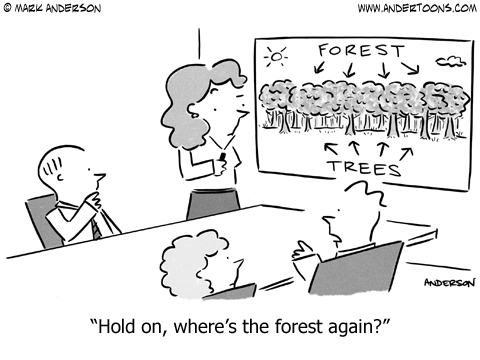
\includegraphics[scale=.4]{forest_tree_cartoon}
\end{center}
It is easy in a statistics class to focus on the specifics. I want you to remember why we are doing what we are doing.

}


\section{Univariate Descriptive Statistics}


\frame{
\frametitle{Binary Data}

\begin{table}[h]
\begin{center}
\caption{Population}\label{t:sam}
\begin{tabular}{r|rrrrrr|r}
$i$ & 1 & 2 & 3 & 4 & $\dots$ & 625 & $\bar{y}_{625}$  \\
$y_i$ & 1 & 1 & 0 & 1 & $\dots$ & 0 & .68 \\
\end{tabular}
\end{center}
\end{table}


Without covariates (and if the indexes aren't otherwise informative), $n$ and $p$ contain all the information.\\

\bigskip

What about data with more values?



}



\frame{
\frametitle{Example: Epstein and Mershon SCOTUS data}

\begin{itemize}
\item Data on 27 justices from the Warren (`53 - `69), Burger (`69 - `86), and Rehnquist (`86 - `05) courts \pause
\item Data can be interpreted as a census for the 1953 - 2005 era.  \pause
\item Percentage of votes in liberal direction for each justice in civil liberties cases
%\item Segal-Cover scores for each justice  \pause
%\item Party of appointing president
\end{itemize}

}

\frame{
\frametitle{Describing Univariate Data}

\begin{figure}[ht] \centering
        \scalebox{.4}{
\includegraphics{CLhist.pdf}}
\end{figure}


}

%\frame{
%\frametitle{Describing Bivariate Data}
%
%\begin{figure}[ht] \centering
%        \scalebox{.4}{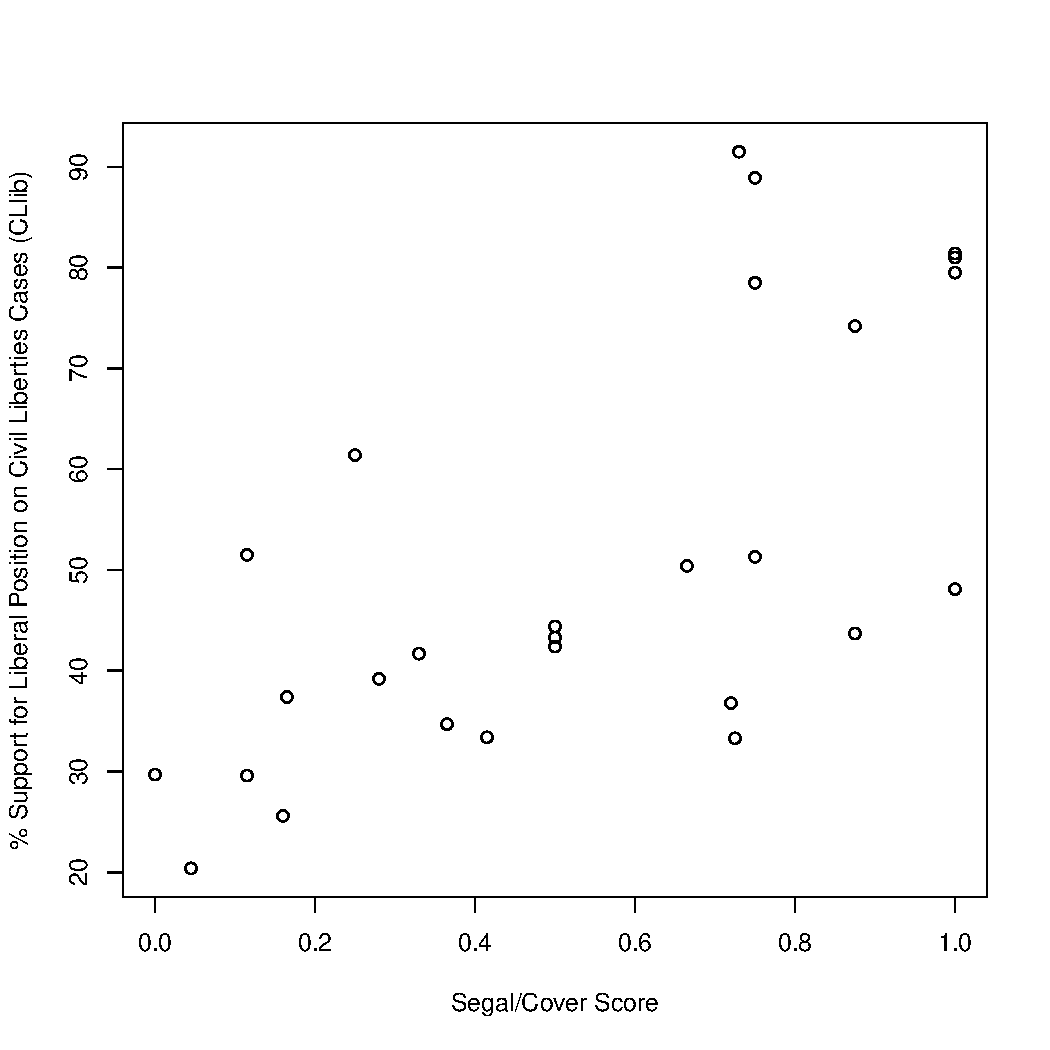
\includegraphics{scat2d.pdf}}
%\end{figure}
%
%
%}
%
%
%\frame{
%\frametitle{Describing Bivariate Data}
%
%\begin{figure}[ht] \centering
%        \scalebox{.4}{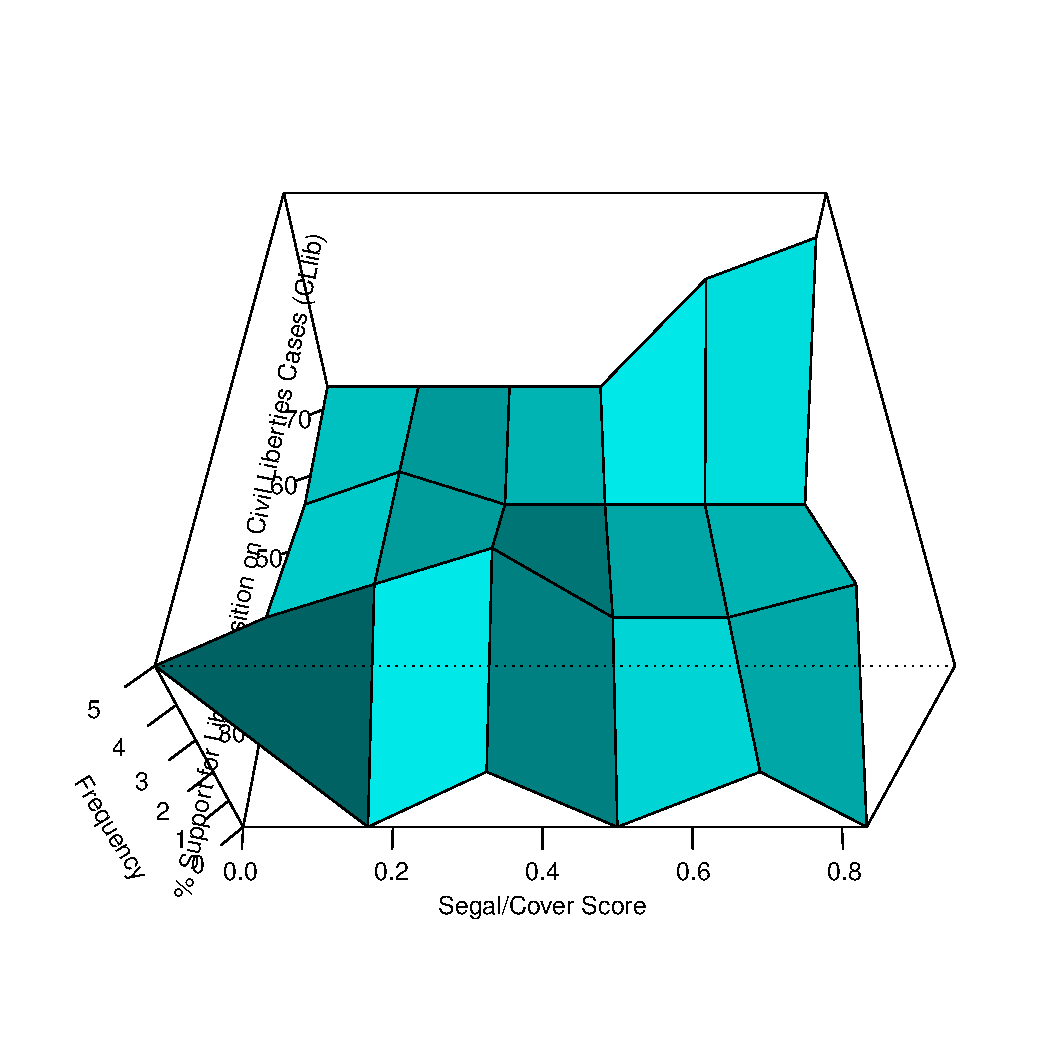
\includegraphics{hist2d.pdf}}
%\end{figure}
%
%
%}
%
%
%\frame{
%\frametitle{Describing Trivariate Data}
%
%\begin{figure}[ht] \centering
%        \scalebox{.4}{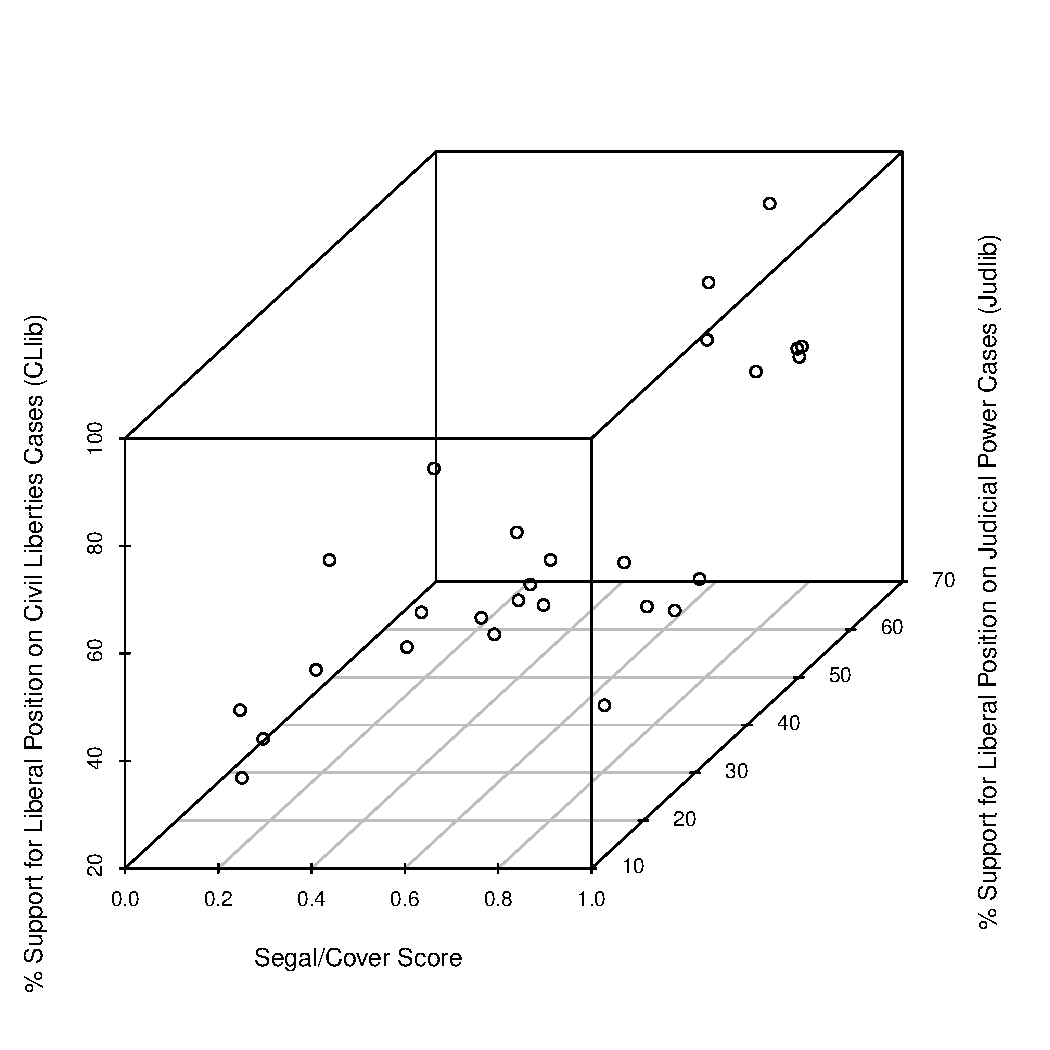
\includegraphics{scat3d.pdf}}
%\end{figure}
%
%}
%


\frame{
\frametitle{Summarization}

\begin{itemize}
\item Even for univariate data, we may want to focus on one or two characteristics of the population instead of describing it in its entirety. \pause
\item We typically focus on measures of center and spread.\pause
\item We will discuss the rational for this over the coming weeks.
\end{itemize}
}


\frame{
\frametitle{Univariate Activity}

\begin{figure}[ht] \centering
        \scalebox{.4}{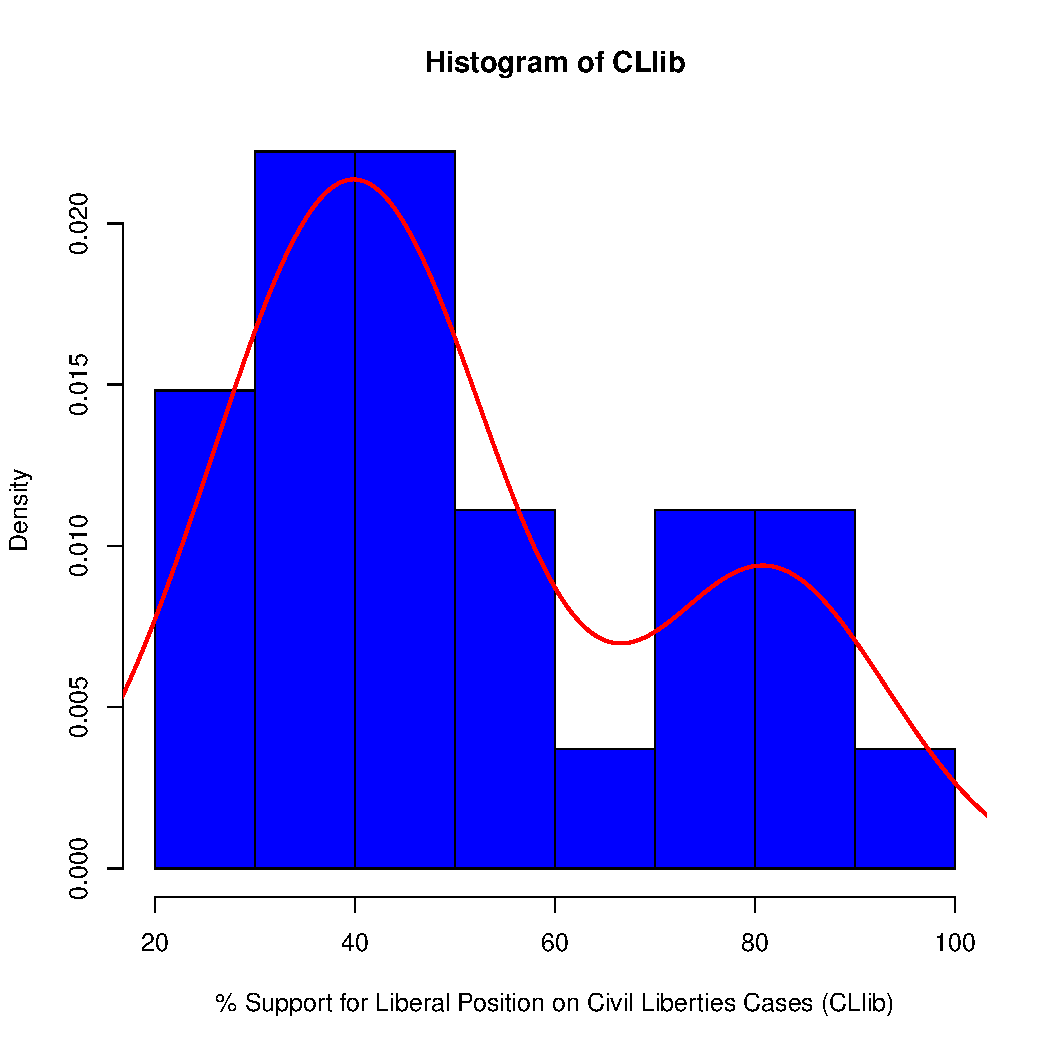
\includegraphics{CLhistAct.pdf}}
\end{figure}
\centering Find the rough location of the mean and median.
}

\frame{
\frametitle{Univariate Activity Solution}

\begin{figure}[ht] \centering
        \scalebox{.4}{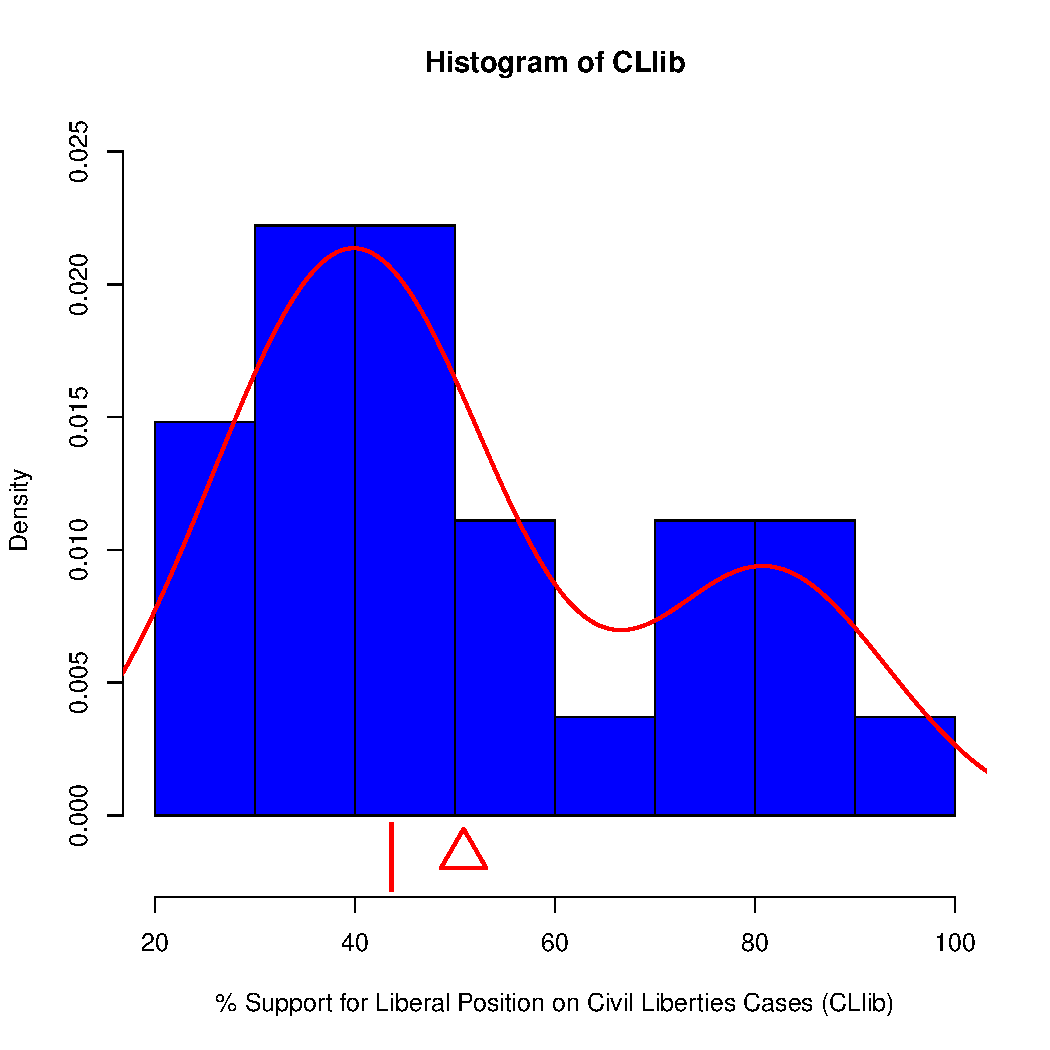
\includegraphics{CLhistActSol.pdf}}
\end{figure}

}

\frame{
\frametitle{Mean as a balance point}
\begin{center}
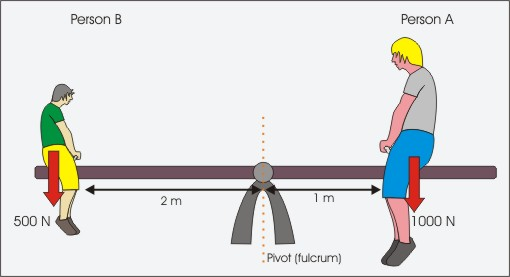
\includegraphics[scale=.5]{seesaw}
\end{center}
}


\frame{
\frametitle{Choosing a descriptive statistic}

How might we choose between these descriptive statistics?

\begin{enumerate}
\item brief: at most a few numbers \pause
\item includes main points: \pause
\begin{itemize}
\item sufficient to describe main characteristics of the data
\item minimizes the information lost by reducing the data
\end{itemize}
\end{enumerate} 



}




\frame{
\frametitle{A Least Squares Summary}

Suppose we want to pick a single number ($m$) for the middle of the data that summarizes all the values for $y$, by minimizing the sum of squared residuals (i.e., least squares).
$$
SSR(\tilde{m}) = \sum_{i=1}^N (y_i - \tilde{m})^2.
$$
\pause

Activity: Using calculus, derive the least squares estimator
\begin{enumerate}
  \item Calculate the derivative of $SSR$ with respect to $\tilde{m}$
  \item Set the derivative equal to 0
  \item Solve for $m$
\end{enumerate}

}



\frame{
\frametitle{The Objective Function for SSR CLlib}
\begin{figure}[ht] \centering
        \scalebox{.4}{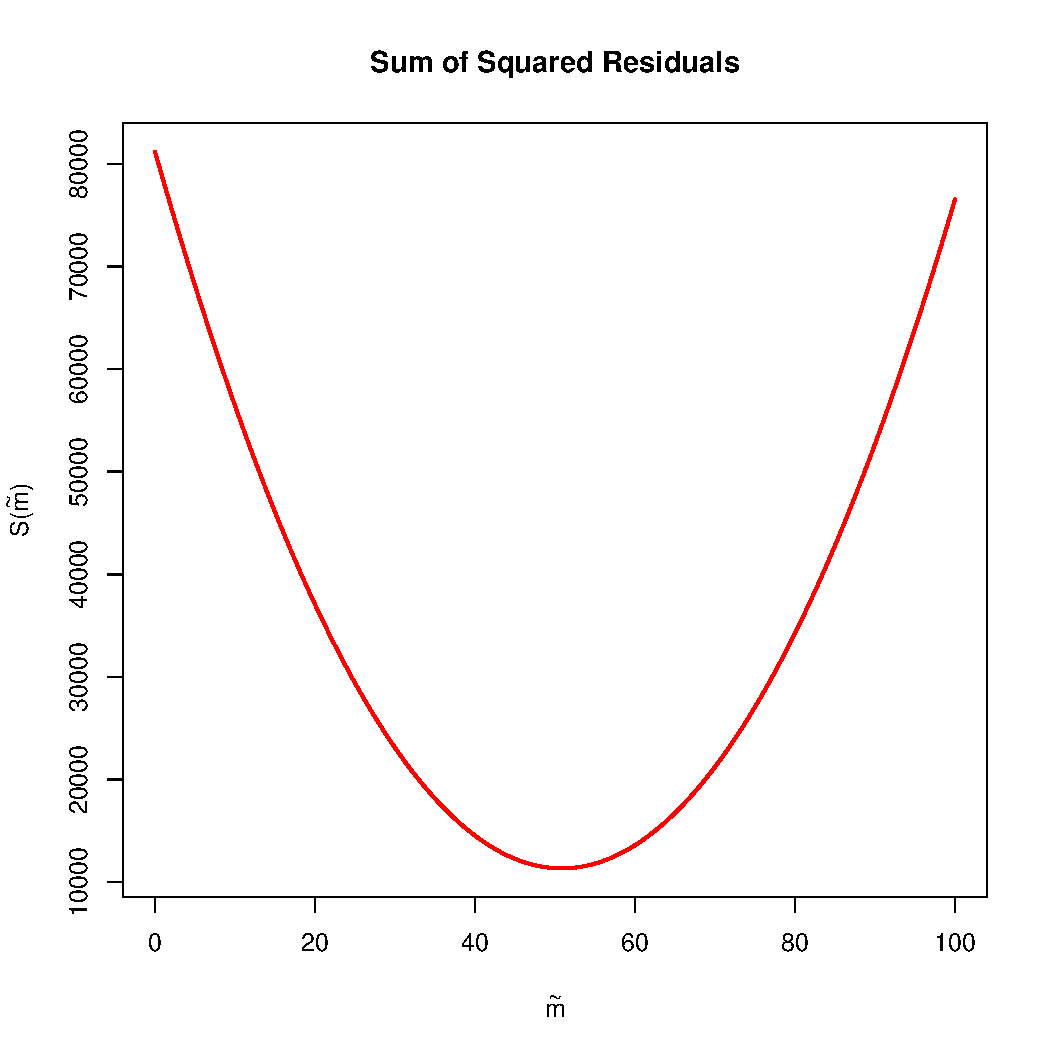
\includegraphics{objectiveFunction1.pdf}}
\end{figure}

}

\frame{

\begin{enumerate}
\item \begin{align*}
SSR(\tilde{m}) 
  &= \sum_{i=1}^N (y_i -
  \tilde{m})^2\\
  &= \sum_{i=1}^N (y_i^2 - 2 y_i \tilde{m} + \tilde{m}^2)
\end{align*} 
 $$
\frac{\partial SSR(\tilde{m})}{\partial
  \tilde{m}} = \sum_{i=1}^N (-2 y_i + 2 \tilde{m})
$$
\end{enumerate}


\vspace{3cm}
}

\frame{
\frametitle{The Slope of the Tangent Line for SSR CLlib}
\begin{figure}[ht] \centering
        \scalebox{.4}{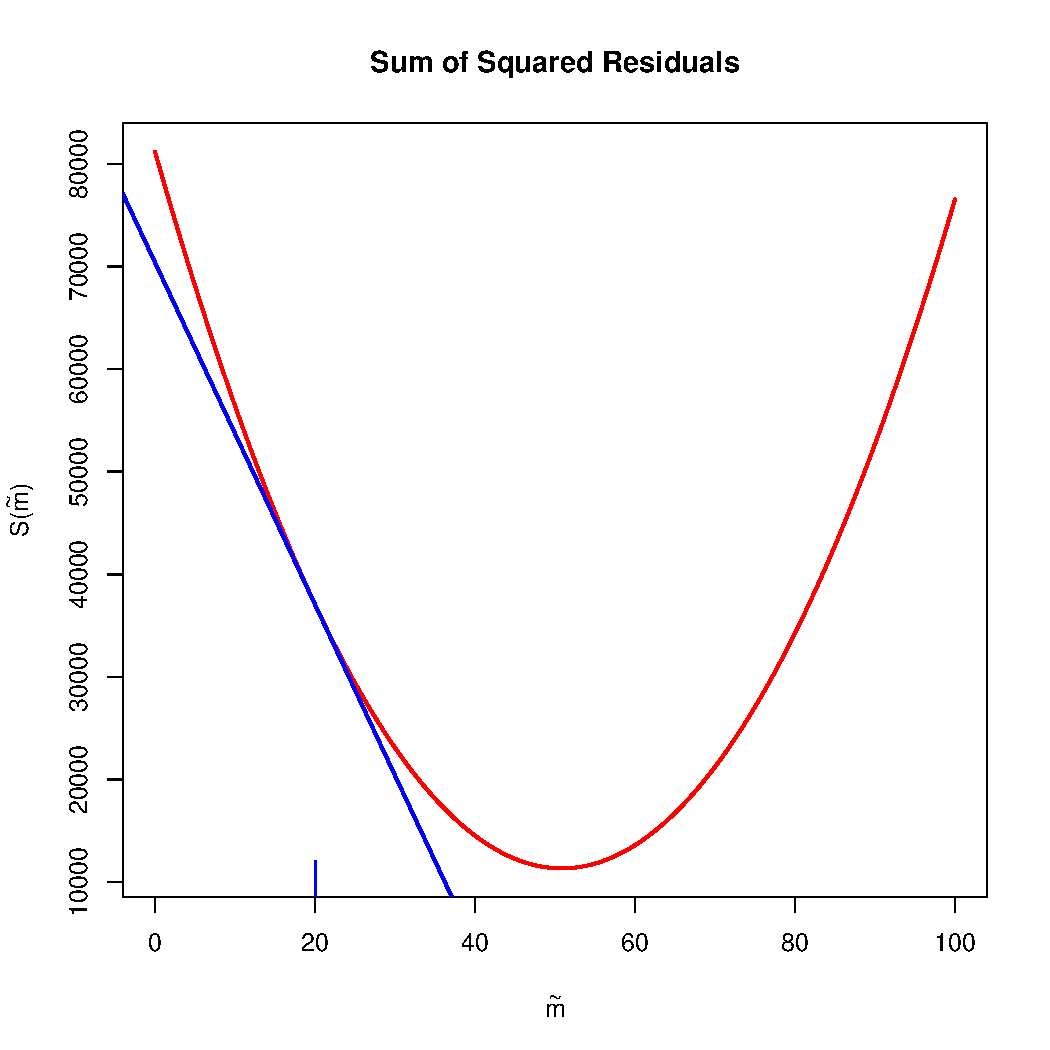
\includegraphics{objectiveFunction2.pdf}}
\end{figure}

}

\frame{
\frametitle{The Slope of the Tangent Line for SSR CLlib}
\begin{figure}[ht] \centering
        \scalebox{.4}{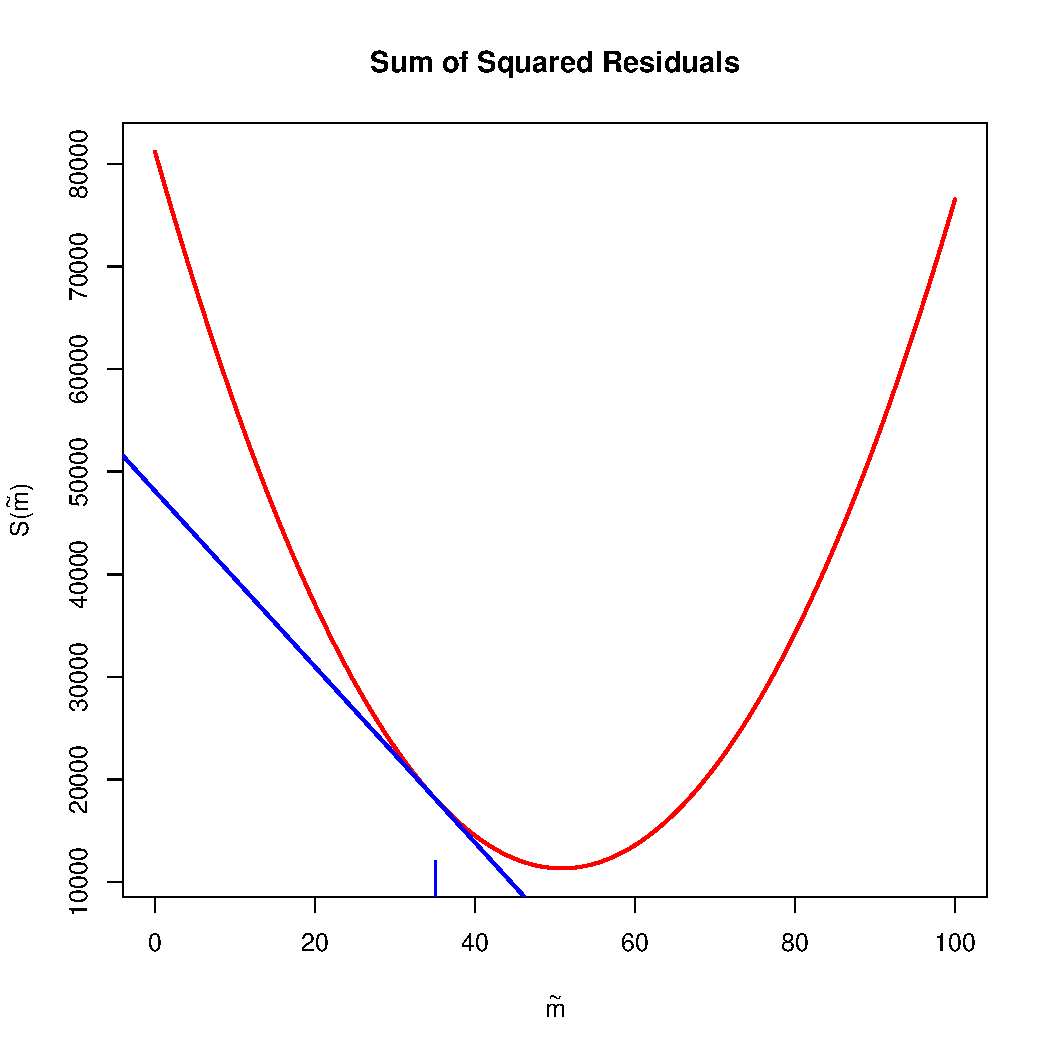
\includegraphics{objectiveFunction3.pdf}}
\end{figure}

}

\frame{
\frametitle{The Slope of the Tangent Line for SSR CLlib}
\begin{figure}[ht] \centering
        \scalebox{.4}{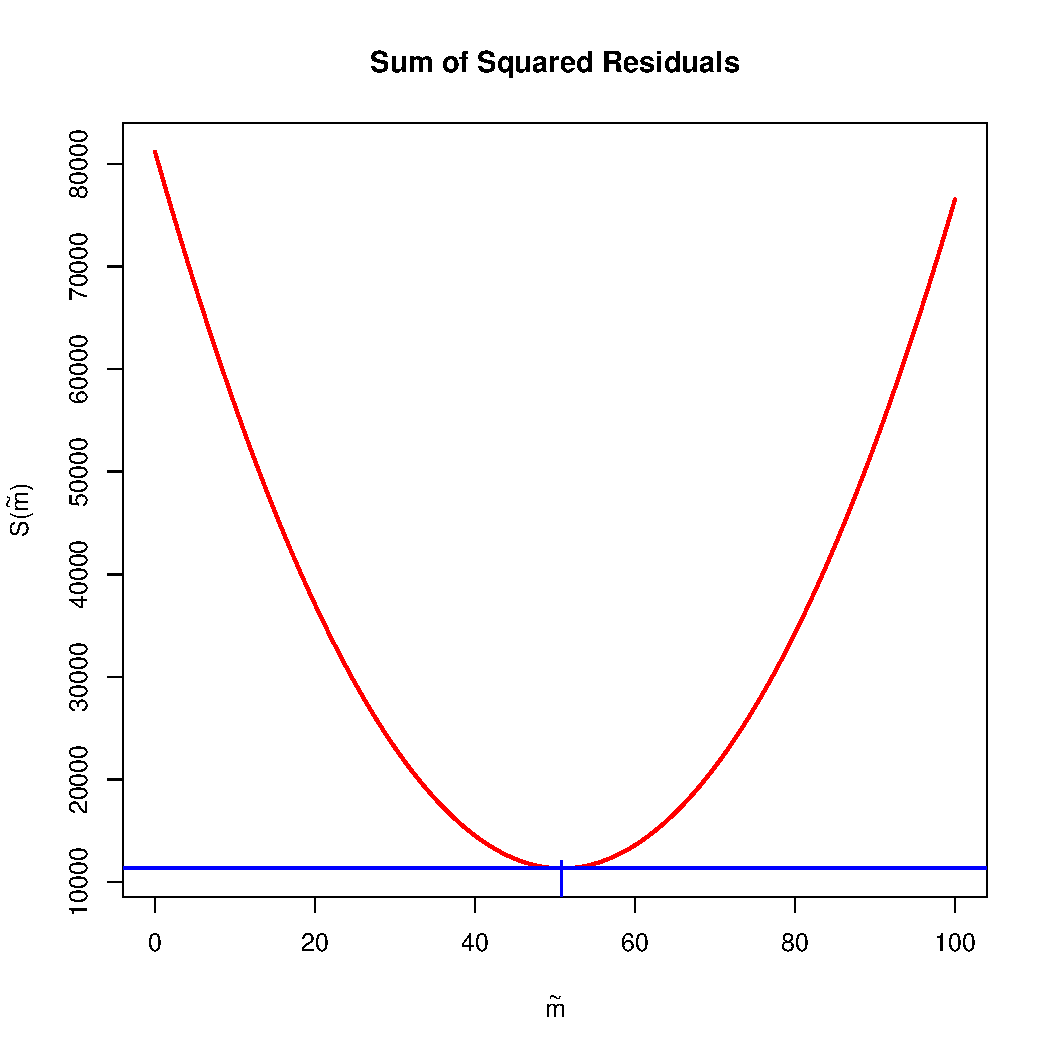
\includegraphics{objectiveFunction4.pdf}}
\end{figure}

}


\frame{

\begin{enumerate}
\item \begin{align*}
SSR(\tilde{m}) 
  &= \sum_{i=1}^N (y_i -
  \tilde{m})^2\\
  &= \sum_{i=1}^N (y_i^2 - 2 y_i \tilde{m} + \tilde{m}^2)
\end{align*} 
 $$
\frac{\partial S(m)}{\partial
  \tilde{m}} = \sum_{i=1}^N (-2 y_i + 2\tilde{m})
$$

\item $$
0 = \sum_{i=1}^N (-2 y_i + 2 m)
$$
\item $$
m = \frac{1}{N}\sum_{i=1}^N  y_i 
$$
\end{enumerate}
\vspace{.1cm}
\centering Therefore, the mean is a least squares summary.

}


\frame{
\frametitle{A Least Absolute Value Summary}

Suppose we want to pick a single number ($m$) for the middle of the data that summarizes all the values for $y$, by minimizing the sum of absolute deviations.
$$
SAV(\tilde{m}) = \sum_{i=1}^N |y_i - \tilde{m}|.
$$
\pause


\begin{itemize}
  \item Why is this harder to solve?
  \item Any guesses?
\end{itemize}

}


\frame{
\frametitle{Why we focus on means}

\begin{itemize}
\item Means often provide a ``good'' summary of the data (and it is relatively easy to tell when they provide bad summaries).  \pause
\item The properties of means are relatively easy to describe.  \pause
\item Sufficient in a sense (in a few slides). \pause
\item Randomized experiments only identify average causal effects (as do regression and matching when the appropriate assumptions hold).
\end{itemize}

}

\frame{
\frametitle{Variance and Standard Deviation}

\begin{itemize}
\item Mean is the least squares predictor in terms of SSR.
\item How small is ``least'' (i.e., how much spread around the mean)?
\item Variance and Standard Deviation are useful transformations of SSR for the mean.
\end{itemize} \pause

Population Variance
\begin{align*}
S^2 &= \frac{\sum_{i=1}^N (y_i-\bar{y})^2}{N-1} \\ 
&=  \frac{SSR}{N-1}
\end{align*} \pause

Population Standard Deviation
\begin{align*}
S &= \sqrt{S^2}
\end{align*}

}

\frame{
\frametitle{Mean and Standard Deviation}

\begin{figure}[ht] \centering
        \scalebox{.4}{
\includegraphics{CLhistMSD.pdf}}
\end{figure}


}

\frame{
\frametitle{Variance as turning force}

\begin{center}
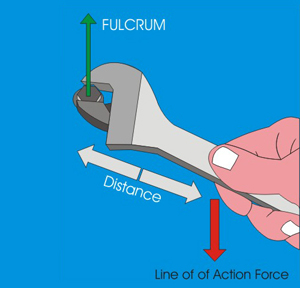
\includegraphics[scale=.5]{turning_effect_01}
\end{center}
}

\frame{
\frametitle{Why variance and standard deviation?}

\begin{itemize}
\item Natural measures of accuracy for means.  \pause
\item Means and variances are sufficient for normally distributed data. \pause
\item For nonnormal data, means and variances provide much information via Chebyshev's inequality and other concentration inequalities. 
\end{itemize}

}

\section{Descriptive Regression with a Coarse Covariate}

\frame{
\frametitle{Conditional Means}

\begin{itemize}
\item In this class, we focus on a single ``outcome'' variable. 
\item All additional variables adjust how we consider the outcome, often by conditioning.
\item Typically, we consider the mean of $y$ conditional on values of other variables.
\end{itemize}

}

\frame{
\frametitle{Binary Outcome with Binary Covariate}

\begin{table}[h]
\begin{center}
\caption{Population}\label{t:sam}
\begin{tabular}{r|rrrrrr|r}
$i$ & 1 & 2 & 3 & 4 & $\dots$ & 625 & mean  \\
$y_i$ & 1 & 1 & 0 & 1 & $\dots$ & 0 & .68 \\
$x_i$ & 1 & 0 & 1 & 0 & $\dots$ & 0 & .5 \\
\end{tabular}
\end{center}
\end{table}

\begin{itemize}
\item Instead of one proportion, we now have two conditional proportions (one for $x=0$ and one for $x=1$).
\item In regression, we focus on conditional means/proportions (not joint proportions).
\end{itemize}

}



\frame{
\frametitle{From Univariate to Regression}

\begin{figure}[ht] \centering
        \scalebox{.4}{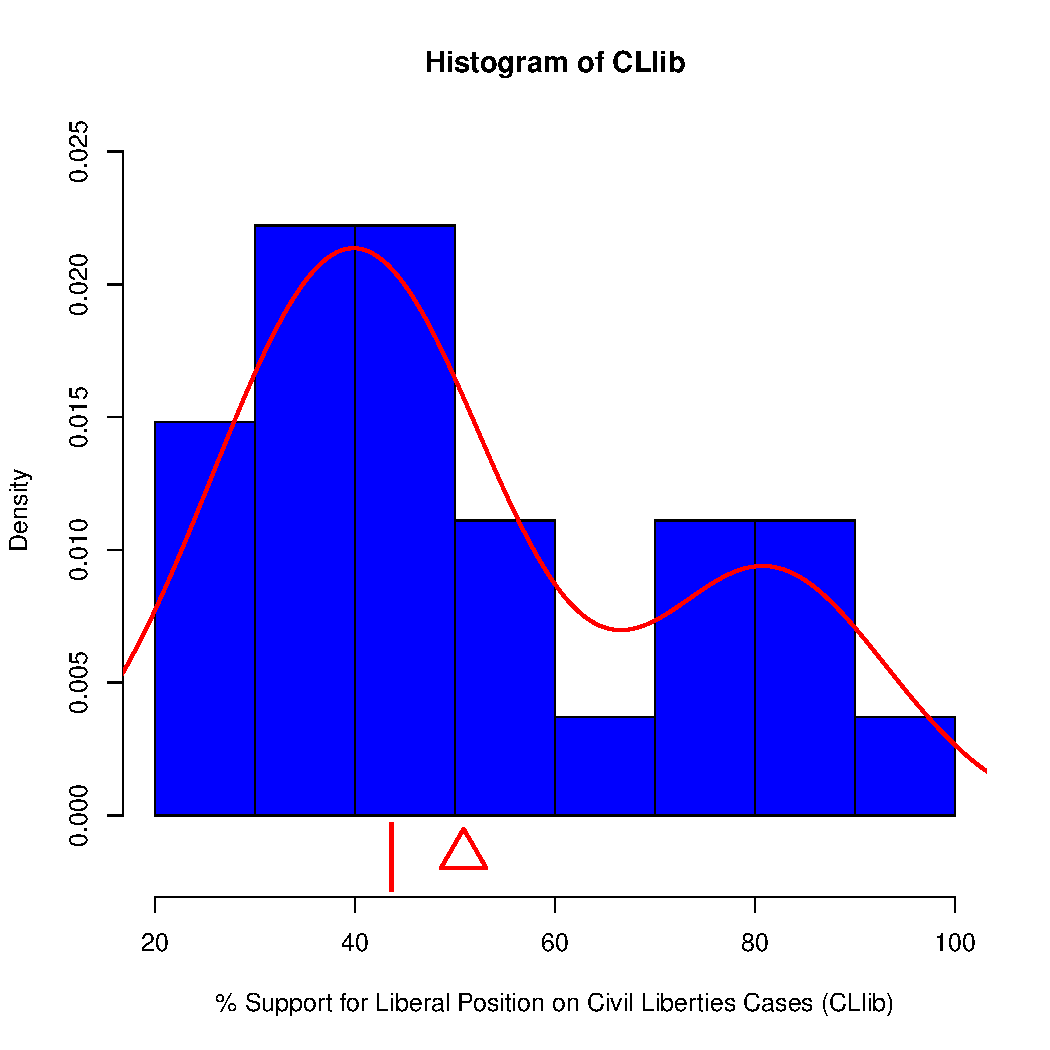
\includegraphics{CLhistActSol.pdf}}
\end{figure}

}


\frame{
\frametitle{From Univariate to Regression}

\begin{figure}[ht] \centering
        \scalebox{.4}{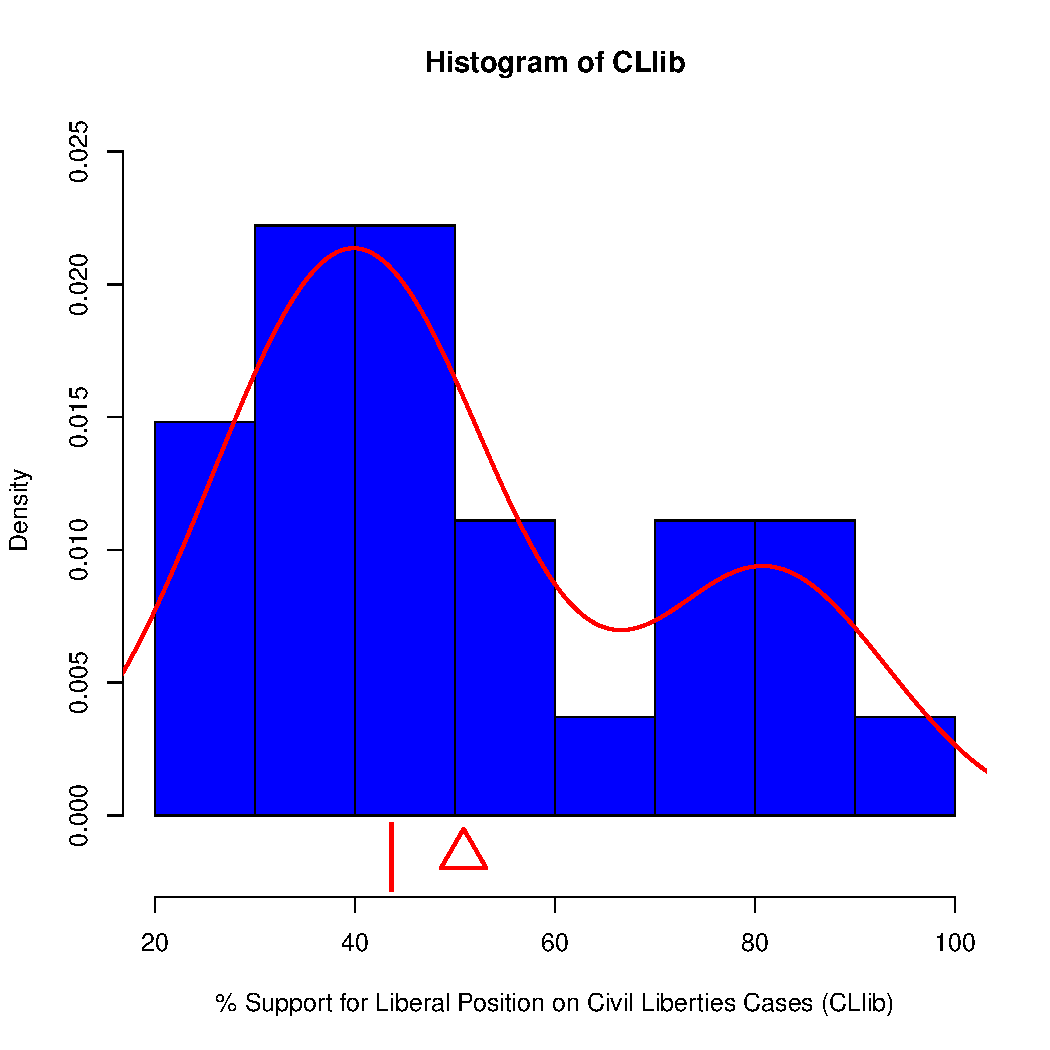
\includegraphics[angle=90,origin=c]{CLhistActSol.pdf}}
\end{figure}

}

\frame{
\frametitle{Mean CLlib Conditional on Party}

\begin{figure}[ht] \centering
        \scalebox{.4}{\includegraphics{partyMean.pdf}}
\end{figure}


}



\frame{
\frametitle{Coarse and Fine-grained Covariates} 

\begin{center}
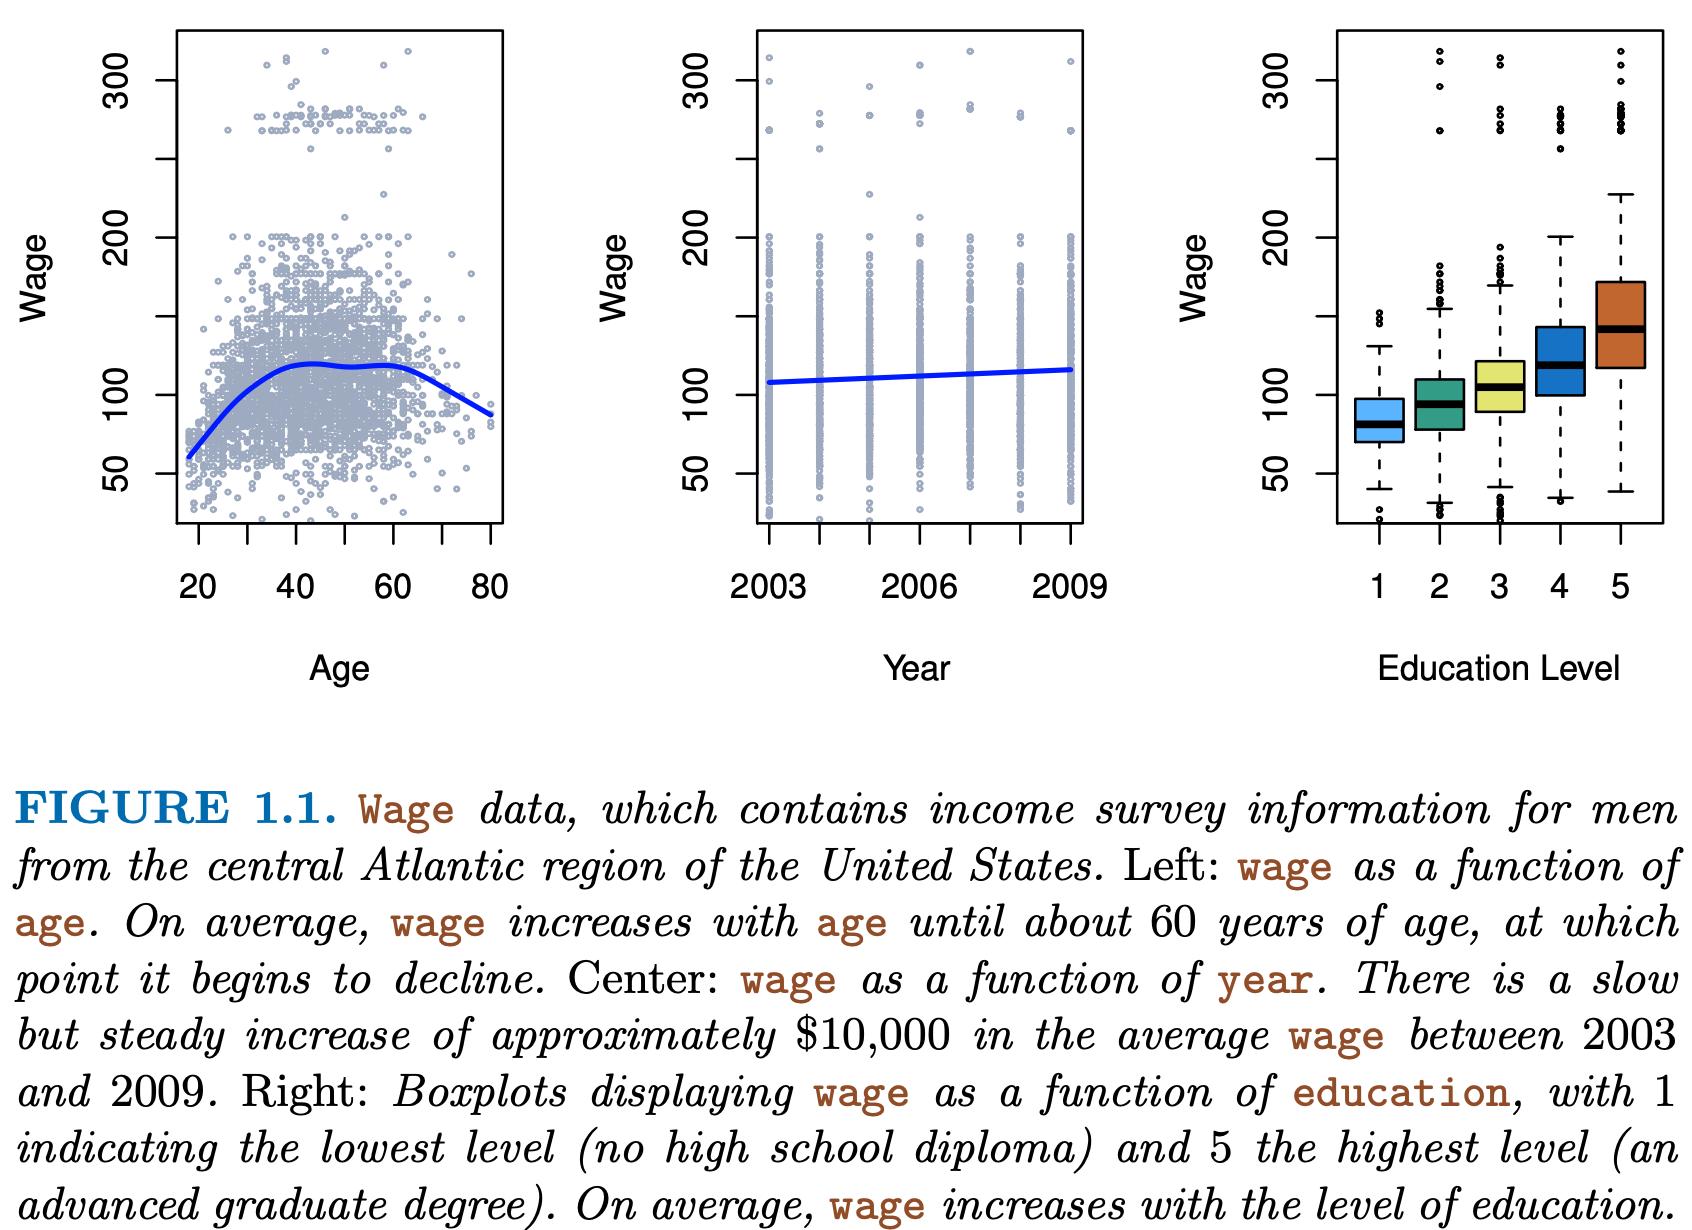
\includegraphics[scale=.33]{CoarseVsFineGrained}
\end{center}
}






\section{Descriptive Linear Regression}



\frame{
\frametitle{Mean CLlib Conditional on Party}

\begin{figure}[ht] \centering
        \scalebox{.4}{\includegraphics{partyMean.pdf}}
\end{figure}


}

\frame{
\frametitle{Linear Conditional Mean Function (LCMF)}

\begin{figure}[ht] \centering
        \scalebox{.4}{
\includegraphics{lmBin.pdf}}
\end{figure}


}

\frame{
\frametitle{What about a continuous explanatory variable?}

\begin{center}
\includegraphics<1>[width=7.25cm]{justicePlot1.pdf}
\includegraphics<2>[width=7.25cm]{justicePlot2.pdf}
%\includegraphics<3>[width=7.25cm]{justicePlot1.pdf}
%\includegraphics<4>[width=7.25cm]{justicePlot3.pdf}
\includegraphics<3>[width=7.25cm]{justicePlot4.pdf}
\end{center}


}




\frame{
\frametitle{Fitted Values and Residuals}

\begin{itemize}
\item Fitted Values from LCMF: $\alert{\hat{y}_i} = B_0 + B_1 x_i$ for $i=1,...,N$ 
\item Residuals from Fitted Values:  $\textcolor{green}{e_i} = y_i - \hat{y}_i$ for $i=1,...,N$
\end{itemize}

\vspace{-.25cm}

\begin{center}
\includegraphics<1>[width=7cm]{fitted.pdf}
\includegraphics<2>[width=7cm]{fitted2.pdf}
\includegraphics<3>[width=7cm]{residuals.pdf}
\end{center}
}

\frame{
\frametitle{Minimizing the Residuals}

%Intuitively, we want to "minimize" the residuals. However, any line through the point of averages

\begin{itemize}
\item Let $\tilde{B}_0$ and $\tilde{B}_1$ be possible values for $B_0$ and $B_1$ respectively,
    \item \emph{Least Squares (LS) regression}: 
    $$
    (B_0, B_1) =   
     \underset{\tilde{B}_0, \tilde{B}_1}{\textrm{argmin}}
    \sum_{i=1}^N (y_i - \tilde{B}_0 - x_i \tilde{B}_1)^2
    $$ 
\end{itemize}

}

\frame{
\frametitle{Simple Regression Activity}

\begin{center}
\includegraphics<1>[width=7.25cm]{simRegAct.pdf}
\includegraphics<2>[width=7.25cm]{simRegActSol.pdf}

\end{center}

}

\frame{
\frametitle{Choosing Slope and Intercept to Minimize SSR}

\begin{figure}[ht] \centering
        \scalebox{.45}{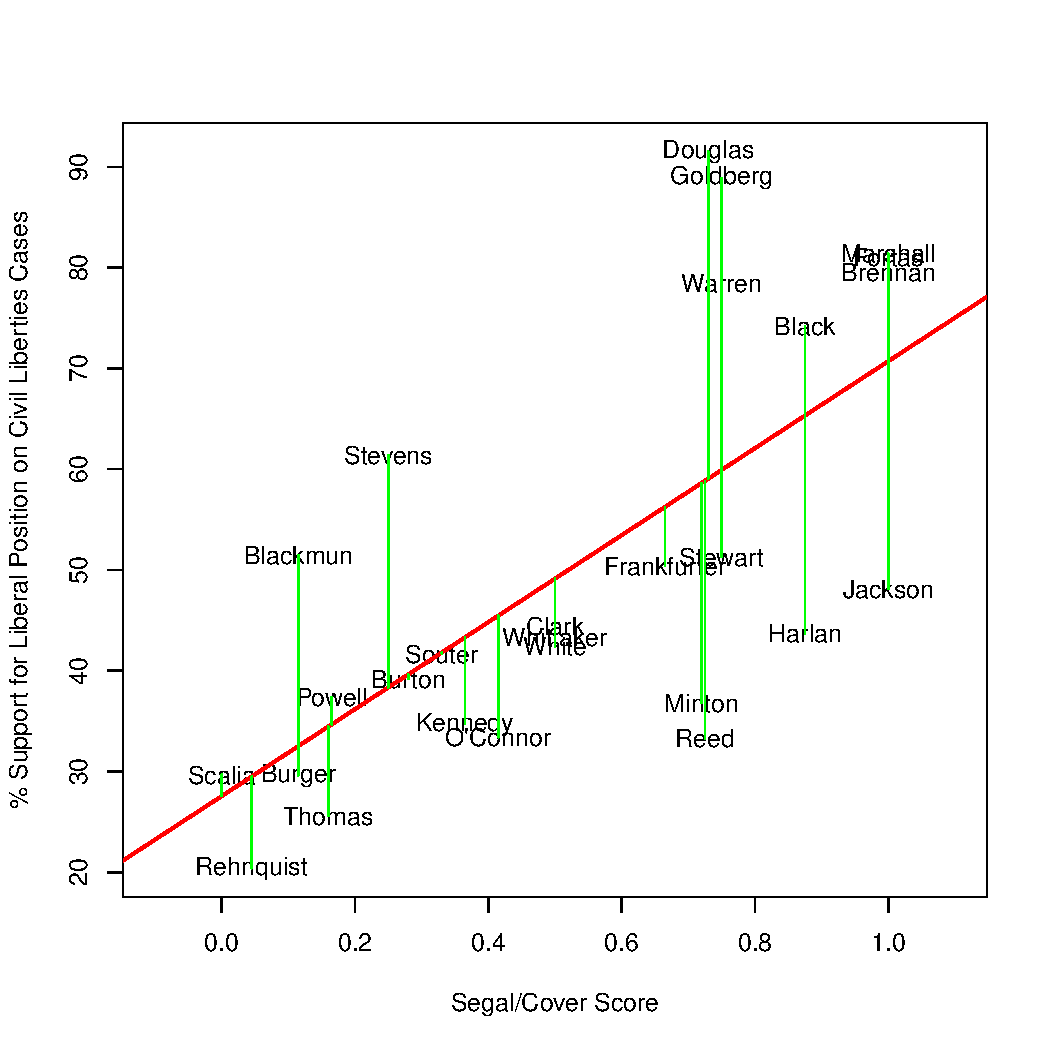
\includegraphics{residuals.pdf}}
\end{figure}

}


\frame{
\frametitle{Deriving the Linear Least Squares Estimator}

Let $\tilde{B}_0$ and $\tilde{B}_1$ be possible values for $B_0$ and $B_1$ respectively, and 
$$
S(\tilde{B}_0, \tilde{B}_1) = \sum_{i=1}^N (y_i -
\tilde{B}_0 - x_i \tilde{B}_1)^2.
$$


\begin{enumerate}
  \item  Take partial derivatives of $S$ with respect to
    $\tilde{B}_0$ and $\tilde{B}_1$. 
  \item Set each of the partial derivatives to 0
  \item Substitute $B_0$ and $B_1$ for
    $\tilde{B}_0$ and $\tilde{B}_1$ and solve for
    $B_0$ and $B_1$
\end{enumerate}

}


%\frame{
%\frametitle{The Objective Function for OLS}
%\begin{figure}[ht] \centering
%        \scalebox{.4}{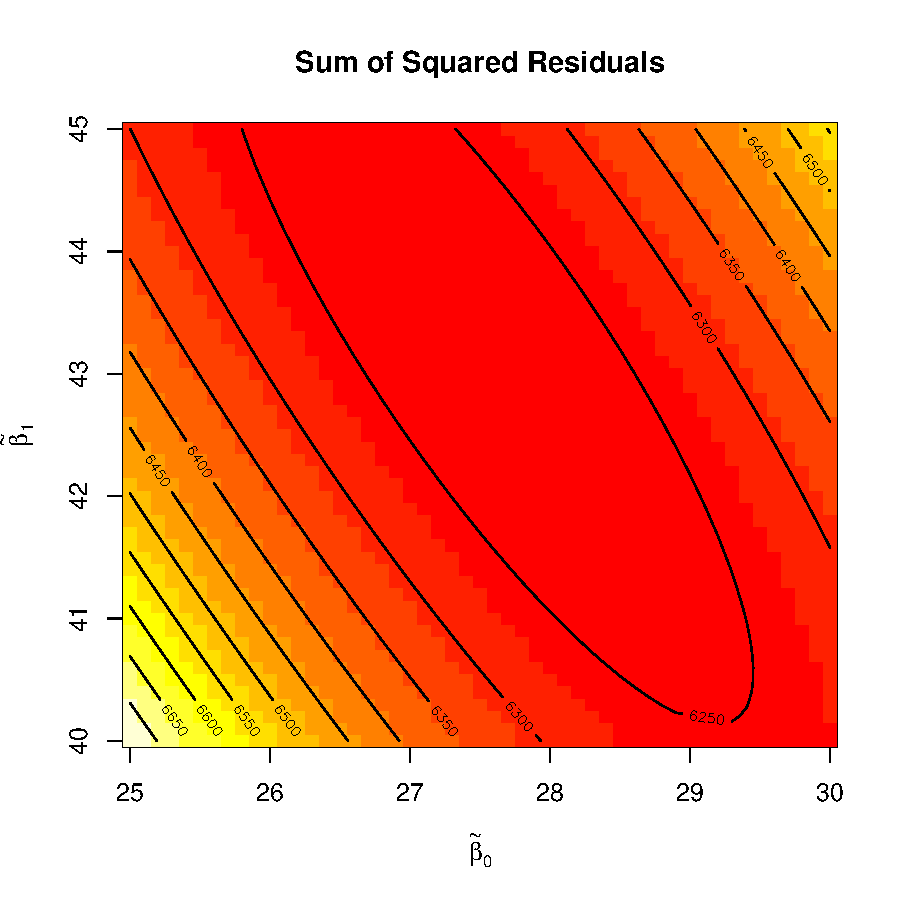
\includegraphics{OLSobjectiveFunction1.pdf}}
%\end{figure}
%
%}
%
%\frame{
%\frametitle{The Objective Function for OLS}
%\begin{figure}[ht] \centering
%        \scalebox{.4}{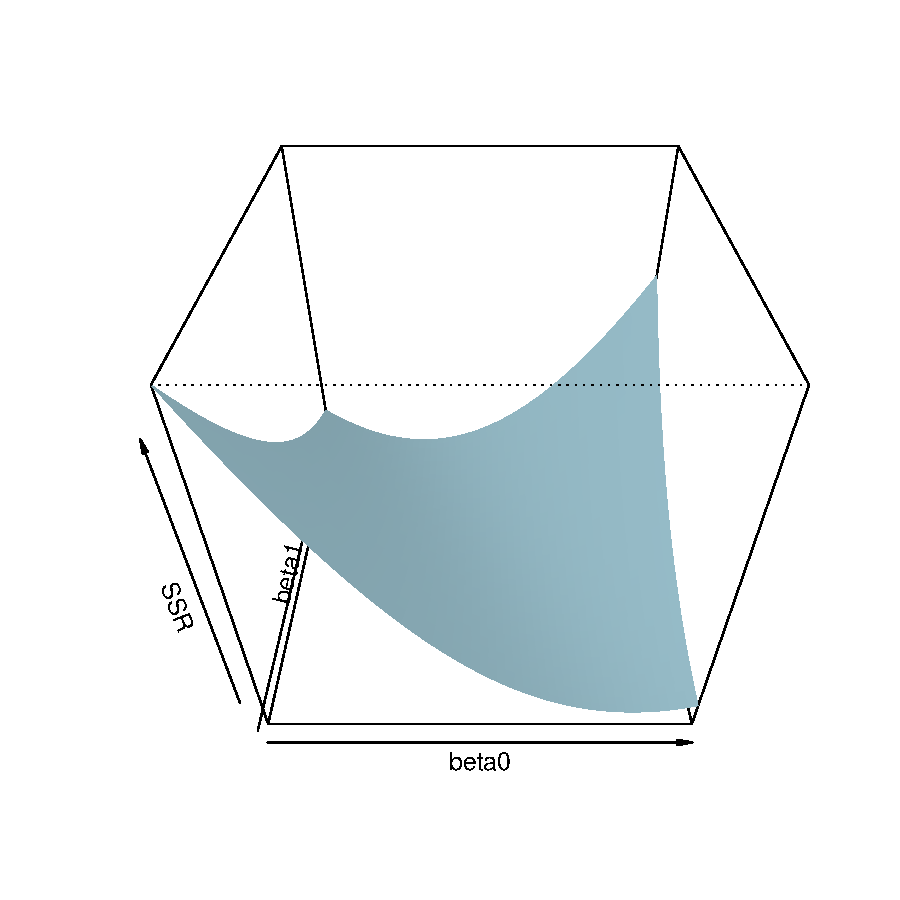
\includegraphics{OLSobjectiveFunction2.pdf}}
%\end{figure}
%
%}


%\frame{

%\begin{align*}
%S(\tilde{\beta}_0, \tilde{\beta}_1) 
%  &= \sum_{i=1}^n (y_i -
%  \tilde{\beta}_0 - x_i \tilde{\beta}_1)^2\\
%  &= \sum_{i=1}^n (y_i^2 - 2 y_i \tilde{\beta}_0 - 2 y_i
%  \tilde{\beta}_1 x_i + \tilde{\beta}_0^2 + 2 \tilde{\beta}_0
%  \tilde{\beta}_1 x_i + \tilde{\beta}_1^2 x_i^2)
%\end{align*} 

%

%$$
%\frac{\partial S(\tilde{\beta}_0, \tilde{\beta}_1)}{\partial
%  \tilde{\beta}_0} = \sum_{i=1}^n (-2 y_i + 2 \tilde{\beta}_0 + 2
%\tilde{\beta}_1 x_i)
%$$
%and 
%$$
%\frac{\partial S(\tilde{\beta}_0, \tilde{\beta}_1)}{\partial
%  \tilde{\beta}_1} = \sum_{i=1}^n (-2 y_i x_i + 2 \tilde{\beta}_0 x_i
%+ 2 \tilde{\beta}_1 x_i^2)
%$$

%}

\frame{



%$$
%\hat{\beta}_0 n = \left(\sum_{i=1}^n y_i\right) - \hat{\beta}_1
%\left(\sum_{i=1}^n x_i\right)  
%$$
%$$
%\hat{\beta}_1 \sum_{i=1}^n x_1^2 = \left(\sum_{i=1}^n x_i y_i\right) -
%\hat{\beta}_0 \left(\sum_{i=1}^n x_i\right)
%$$
%These two \alert{normal equations} imply the following two useful relationships:

\frametitle{Useful Results}
The partial derivatives imply that
$$
\sum_{i=1}^N x_i e_i = 0
$$
$$
\sum_{i=1}^N \hat{y}_i e_i = 0
$$
and the \alert{LS LCMF}:
$$
B_0 = \bar{y} - B_1 \bar{x}
$$
$$
B_1 = \frac{\sum_{i=1}^N (x_i - \bar{x})(y_i -
  \bar{y})}{\sum_{i=1}^N(x_i - \bar{x})^2}
$$
%and one more useful fact:
%$$
%\hat{\beta}_1 = \frac{\sum_{i=1}^n (x_i - \bar{x})y_i}{\sum_{i=1}^n(x_i - \bar{x})^2} - \frac{\sum_{i=1}^n (x_i - \bar{x})
 % \bar{y}}{\sum_{i=1}^n(x_i - \bar{x})^2} =  \frac{\sum_{i=1}^n (x_i - \bar{x})y_i}{\sum_{i=1}^n(x_i - \bar{x})^2}
%$$
}

%\frame{
%\frametitle{The Objective Function for OLS}
%\begin{figure}[ht] \centering
%        \scalebox{.4}{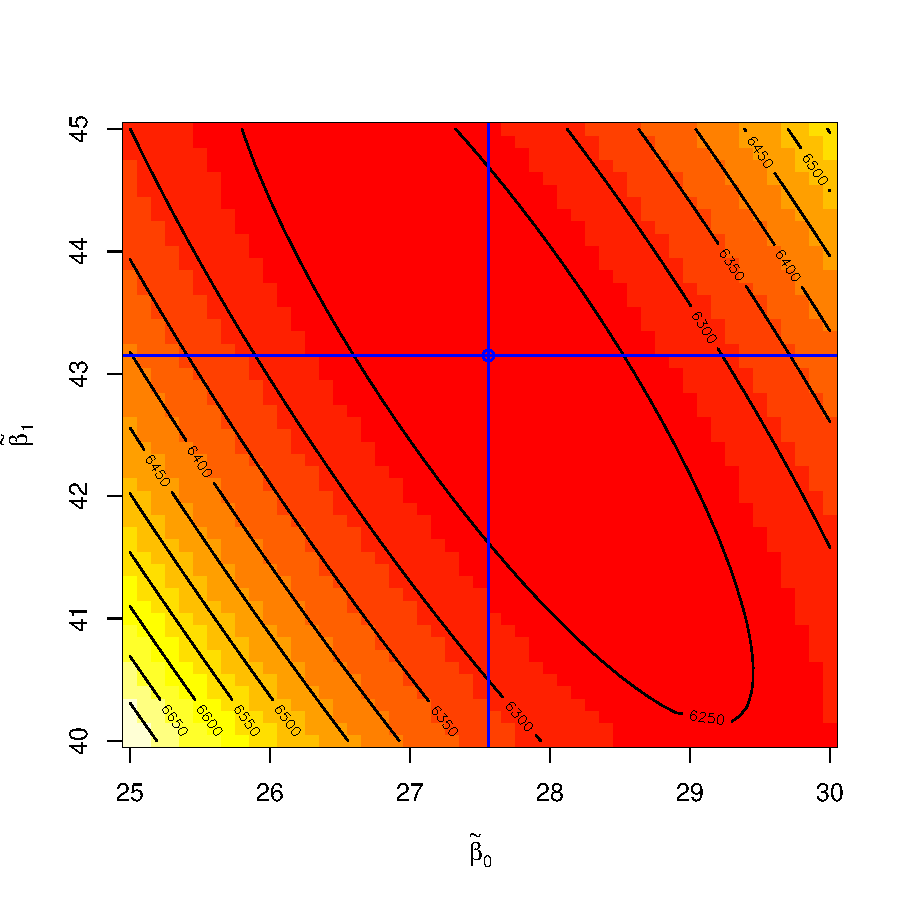
\includegraphics{OLSobjectiveFunction3.pdf}}
%\end{figure}
%
%}


\frame{
\frametitle{Descriptive Interpretation}

\begin{figure}[ht] \centering
        \scalebox{.4}{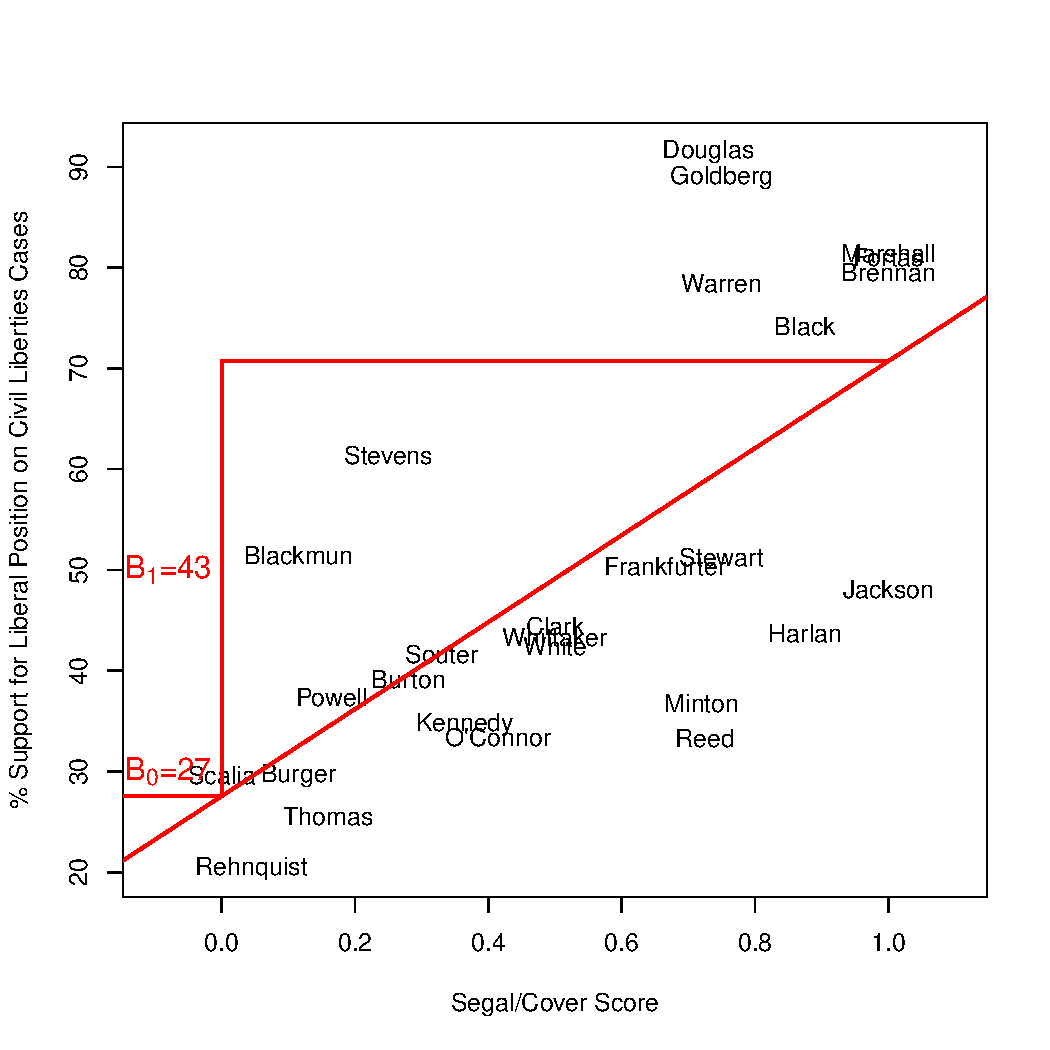
\includegraphics{lmPlot.pdf}}
\end{figure}
%$$
%\hat{\beta}_0 = 27.56 \text{ and } \hat{\beta}_1 = 43.15
%$$ 
}

%%%%%%%%%%%%%%
%\subsection{Goodness of Fit}

\frame{
\frametitle{Variance and Regression}

\begin{itemize}
\item Again, we want to assess the ``leastness'' of  least squares (i.e., the spread of the data around the line).
\item The standard error of the regression, $\sqrt{\frac{\sum_{i=1}^N e_i^2}{N-2}}$, is analogous to the standard deviation.
\item There are other approaches to this question: correlation and coefficient of determination.
\end{itemize}

}


\frame{
\frametitle{Covariance}

The population variances for $X$ and $Y$ can be written as:
\pause
\begin{align*}
S^2_{x} &= \frac{\sum_{i=1}^N (x_i-\bar{x})^2}{N-1} \\ \pause
&= \frac{\sum_{i=1}^N (x_i-\bar{x})(x_i-\bar{x})}{N-1}
\end{align*}
\pause
$$
S^2_{y} = \frac{\sum_{i=1}^N (y_i-\bar{y})(y_i-\bar{y})}{N-1}
$$


\visible<4->{What if we defined a similar quantity involving both $X$ and $Y$?}

\visible<5->{$$
S_{xy} = \frac{\sum_{i=1}^N (x_i-\bar{x})(y_i-\bar{y})}{N-1}
$$}

\visible<6->{This quantity is the \alert{covariance}.}

}

%\frame{
%\frametitle{Properties of Sample Covariance}
%
%	\begin{columns}
%		\begin{column}{.5\textwidth}
%$$
%s_{xy} = \frac{\sum_{i=1}^n (x_i-\bar{x})(y_i-\bar{y})}{n-1}
%$$
%
%\vspace{.15in}
%\pause
%Points in the upper right and lower left quadrants (relative to the means) add to the covariance.
%
%\vspace{.15in}
%\pause
%Points in the upper left and lower right quadrants subtract from the covariance.
%
%		\end{column}
%		\begin{column}{.5\textwidth}
%
%\begin{center}
%\includegraphics<1>[width=2in]{covbase.pdf}
%\includegraphics<2>[width=2in]{covpos.pdf}
%\includegraphics<3>[width=2in]{covneg.pdf}
%\includegraphics<4>[width=2in]{covend.pdf}
%\end{center}
%
%
%		\end{column}
%	\end{columns}
%
%}
%


\frame{
\frametitle{Correlation}

The covariance does not have units that are easy to interpret, so we can scale it by the standard deviations of $X$ and $Y$ to obtain the \alert{correlation}:

$$
R =\frac{S_{xy}}{S_{x}S_{y}}= \frac{\sum_{i=1}^N (x_i-\bar{x})(y_i-\bar{y})}{\sqrt{ \sum_{i=1}^N (x_i-\bar{x})^2  \sum_{i=1}^N (y_i-\bar{y})^2 }}
$$ 
\vspace{.2cm}

\pause
The correlation is always in the interval:
$$
-1 \le R \le 1
$$

}

\frame{
\frametitle{Analysis of Variance for the Regression}

How well do the Segal-Cover scores predict support for civil liberties in relation to the average support for civil liberties?
	\begin{columns}
		\begin{column}{.5\textwidth}
\begin{itemize}
\pause
\item  \textcolor{green}{$e_i = y_i -\widehat{y}_i$}
\pause
\item \textcolor{blue}{$y_i - \bar{y}$}
\pause
\item \textcolor{red}{$\widehat{y}_i - \bar{y}$}
\pause
\item \textcolor{blue}{$(y_i - \bar{y})$} $=$ \textcolor{green}{$e_i$} + \textcolor{red}{$(\widehat{y}_i - \bar{y})$}
\end{itemize}
		\end{column}
		\begin{column}{.5\textwidth}

\begin{center}
	\includegraphics<1>[width=2in]{emlmline.pdf}
	\includegraphics<2>[width=2in]{emresid.pdf}
	\includegraphics<3>[width=2in]{emmeandev.pdf}
	\includegraphics<4>[width=2in]{empred.pdf}
	\includegraphics<5>[width=2in]{emall.pdf}
\end{center}

		\end{column}
	\end{columns}

}

\frame{

\begin{eqnarray*}
\alert<6>{\sum_{i=1}^N(y_i - \bar{y})^2} &=& \sum_{i=1}^N \{e_i + (\widehat{y}_i - \bar{y})\}^2\\
\visible<2->{ &=& \sum_{i=1}^N \{e_i^2 + 2e_i (\widehat{y}_i - \bar{y})+ (\widehat{y}_i - \bar{y})^2\}}\\
\visible<3->{ &=& \sum_{i=1}^N e_i^2 + 2\sum_{i=1}^Ne_i (\widehat{y}_i - \bar{y})+ \sum_{i=1}^N(\widehat{y}_i - \bar{y})^2}\\
\visible<4->{ &=& \alert<7>{\sum_{i=1}^N e_i^2} + \alert<8>{\sum_{i=1}^N(\widehat{y}_i - \bar{y})^2}}\\
\visible<5->{\alert<6>{TSS} &=& \alert<7>{SSR} + \alert<8>{RegSS}}
\end{eqnarray*}

}

\frame{
\frametitle{Coefficient of Determination}

We can divide each side by the TSS:
$$
 \frac{SSR}{TSS} + \frac{RegSS}{TSS} = \frac{TSS}{TSS}
$$
\pause
$$
\frac{SSR}{TSS} + \frac{RegSS}{TSS} = 1
$$
\pause
$$
\frac{RegSS}{TSS} = 1 - \frac{SSR}{TSS} = \alert{R^2}
$$
\pause
$R^2$ is a measure of how much of the variation in $Y$ is accounted for by $X$.
}


\frame{
\frametitle{Usefull Identities}


$$
R^2 = (R)^2
$$

\pause
\begin{eqnarray*}
B_1 &=& \frac{\sum_{i=1}^N (x_i - \bar{x})(y_i -
  \bar{y})}{\sum_{i=1}^N(x_i - \bar{x})^2} \\ 
  & \visible<3->{=}&   \visible<3->{\frac{\sum_{i=1}^N (x_i-\bar{x})(y_i-\bar{y})}{\sqrt{ \sum_{i=1}^N (x_i-\bar{x})^2  \sum_{i=1}^Nn (y_i-\bar{y})^2 }} \cdot \frac{\sqrt{\frac{\sum_{i=1}^N (y_i-\bar{y})^2}{N-1}}}{\sqrt{\frac{\sum_{i=1}^N (x_i-\bar{x})^2}{N-1}}} }\\
  & \visible<4>{=}& \visible<4>{R\frac{S_y}{S_x}}
\end{eqnarray*}

}

\frame{

	\begin{columns}
		\begin{column}{.5\textwidth}

\begin{itemize}

\item $R^2 = 0.45$
\item $R = \sqrt{R^2} = 0.67$
\item $S_x = 0.33$
\item $S_y = 20.9$
\item $B_1 = R\frac{S_y}{S_x} = 43.15$
\end{itemize}

		\end{column}
		\begin{column}{.5\textwidth}

\begin{figure}[ht] \centering
        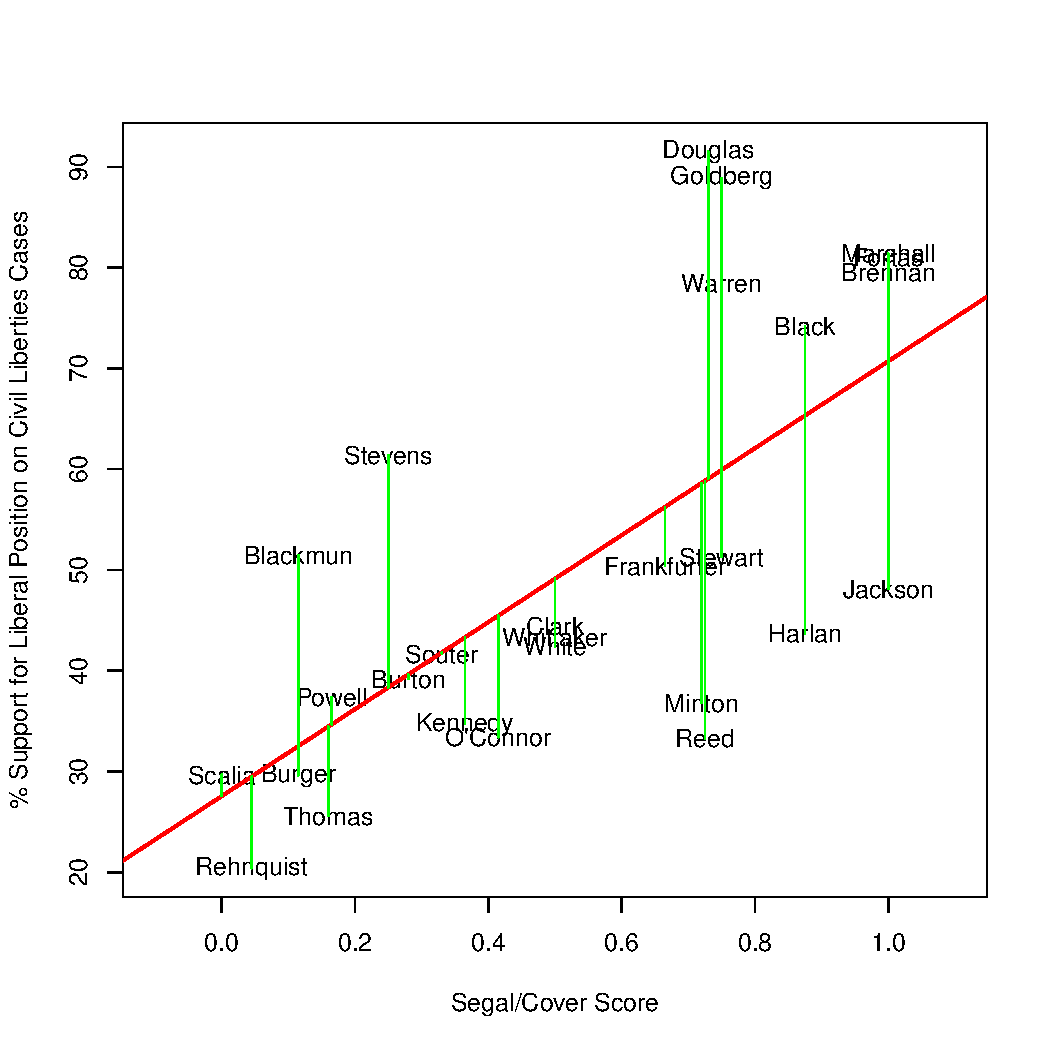
\includegraphics[width=2in]{residuals.pdf}
\end{figure}
		\end{column}
	\end{columns}
}

\frame{
\frametitle{Anscombe's Quartet}

\begin{figure}[ht] \centering
        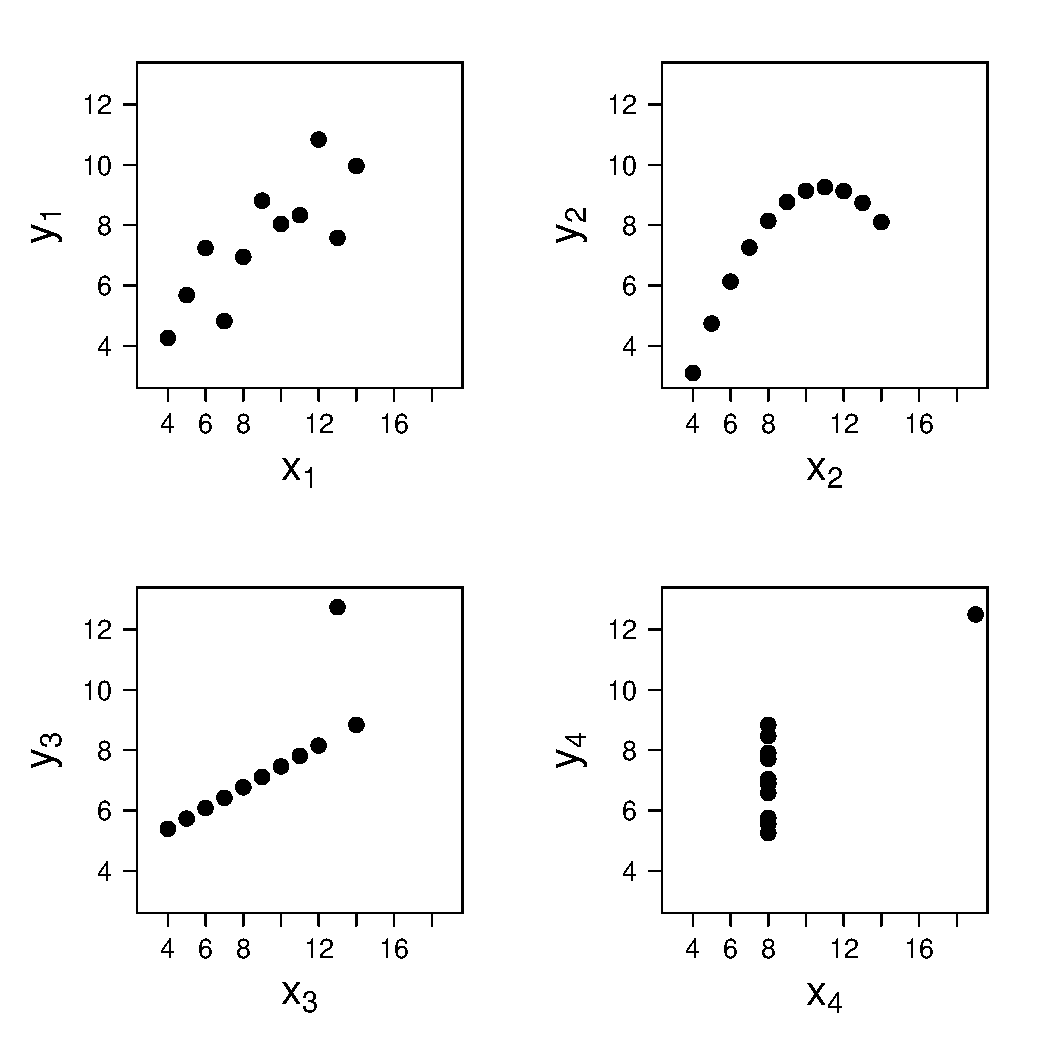
\includegraphics[width=3in]{Anscombe.pdf}
\end{figure}

}

\frame{

	\begin{columns}
		\begin{column}{.5\textwidth}

\begin{figure}[ht] \centering
        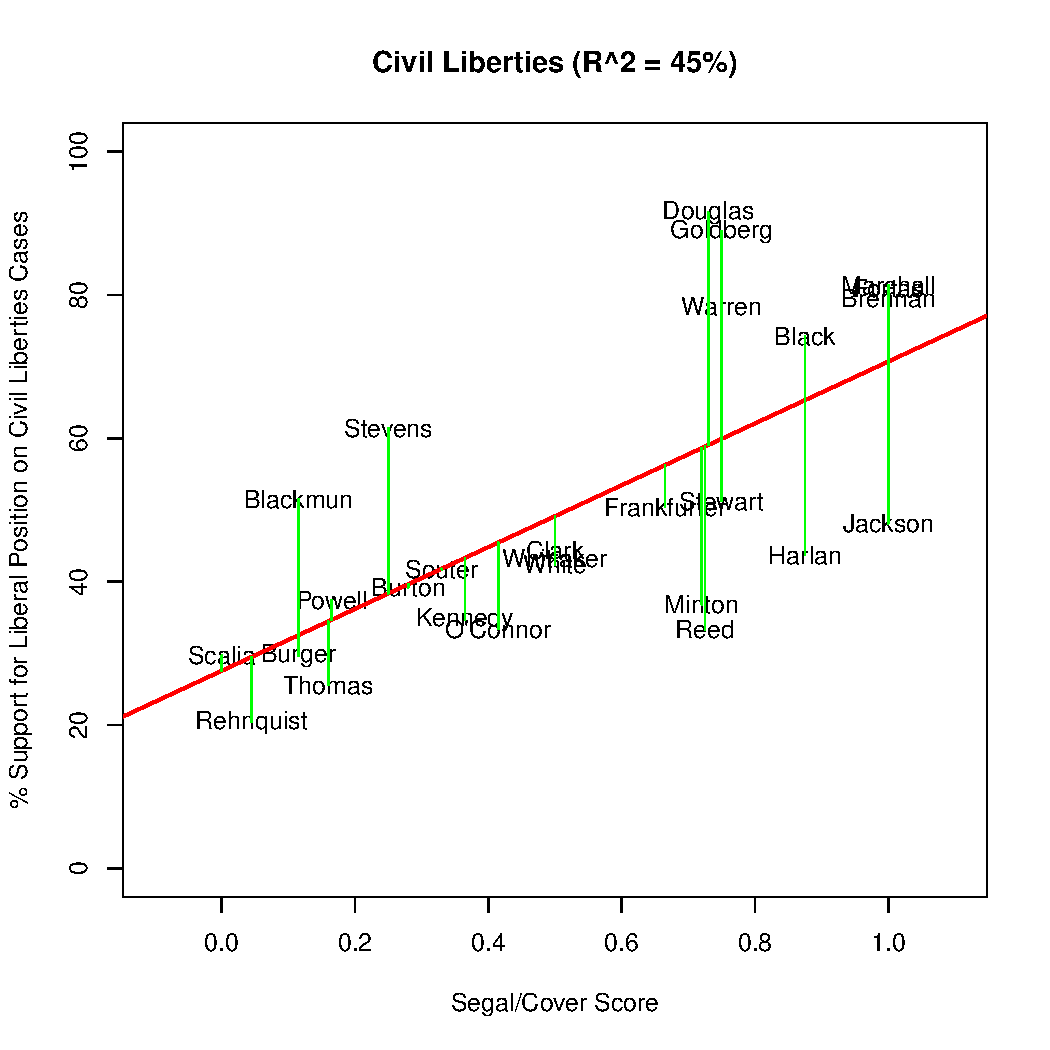
\includegraphics[width=2in]{residuals1.pdf}
\end{figure}
		\end{column}
		\begin{column}{.5\textwidth}

\begin{figure}[ht] \centering
        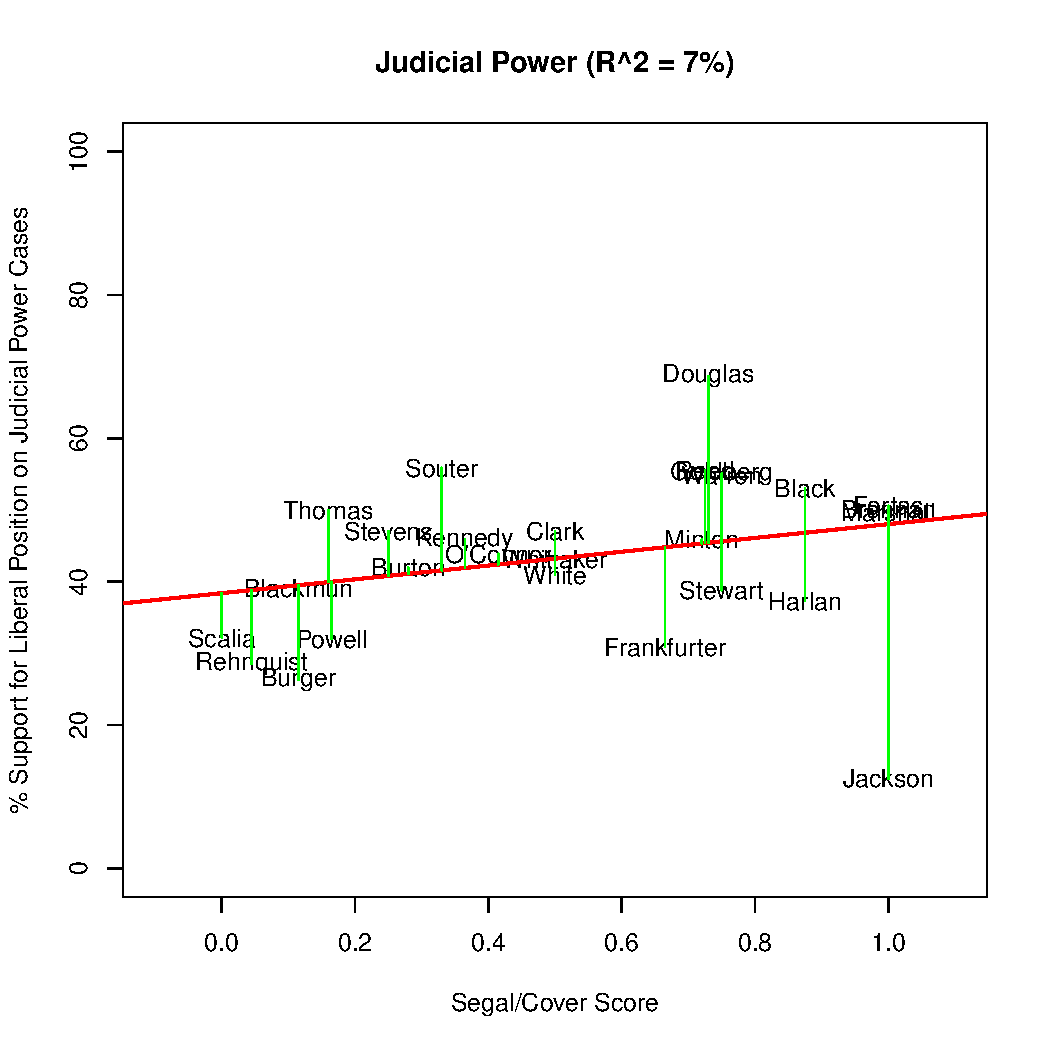
\includegraphics[width=2in]{residuals3.pdf}
\end{figure}
		\end{column}
	\end{columns}
}

\frame{
\frametitle{Tuesday Summary}

\begin{itemize}
\item We will focus on conditional means as a good conditional summary of a single outcome variable.
\item Conditional means are straightforward for a coarse covariate.
\item Linear regression provides a parsimonious summary for a fine-grained covariate.
\end{itemize}

}

\frame{
\frametitle{On Thursday}

\begin{itemize}
\item Binary outcomes with a fine-grained covariate
\item Flexible (i.e., ML) approaches
\end{itemize}

}

%\frame{
%\frametitle{R Activity: Atlanta Science Festival Data}
%
%To do:
%\begin{itemize}
%\item Run linear regression of actual attendance on estimated attendance and discuss the substantive take away from the slope.
%\item Consider adding squared and cubed terms to the regression.
%\item Run leave-one-out cross-validation to compare the models. 
%\end{itemize}
%
%
%}

%\frame{
%	\frametitle{Question:}

%Assume that X and Y are measured in the same units.  Under what conditions will the least squares slope from the regression of Y on X be the same as the least squares slope from the regression of X on Y?

%\begin{itemize}
%\item [A)] The slopes are the same when $s_x = s_y$.
%\item [B)]The slopes are the same when $r = \frac{s_y}{s_x}$.
%\item [C)]The slopes are the same when $s_x = 1$.
%\item [D)]The slopes are never the same.
%\end{itemize}
%}


%%%%%%%%%%%%%%%%%%%%


%\section{Description with Multiple Linear Regression}
%
%
%\frame{
%\frametitle{More Than One Conditioning Variable}
%
%\begin{itemize}
%\item Often we want averages conditional on more than one variable.
%\item As with continuous conditioning variables, there are many ways to do this.
%\item In this class we will look at two.
%\end{itemize}
%
%
%}
%
%\frame{
%\frametitle{Multiple Regression with 2 Conditioning Variables}
%
%\begin{itemize}
%\item Fitted Values from the LCMF $\hat{y}_i = B_0 + B_1 x_i + B_2 z_i$\\
% for $i=1,...,N$ \pause
%\item Residuals from Fitted Values:  $e_i = y_i - \hat{y}_i$ for $i=1,...,N$
%\end{itemize} \pause
%
%\vspace{.5cm}
%
%Again, we choose $B_0$, $B_1$, and $B_2$, to minimize the SSR, where
%\begin{align*}
%SSR &= \sum_{i=1}^N e_i^2
%\end{align*}
%but the definition of $e_i$ changes with the inclusion of more variables. 
%}
%\frame{
%\frametitle{One Binary and One Continuous Conditioning Variable}
%
%\begin{figure}[ht] \centering
%        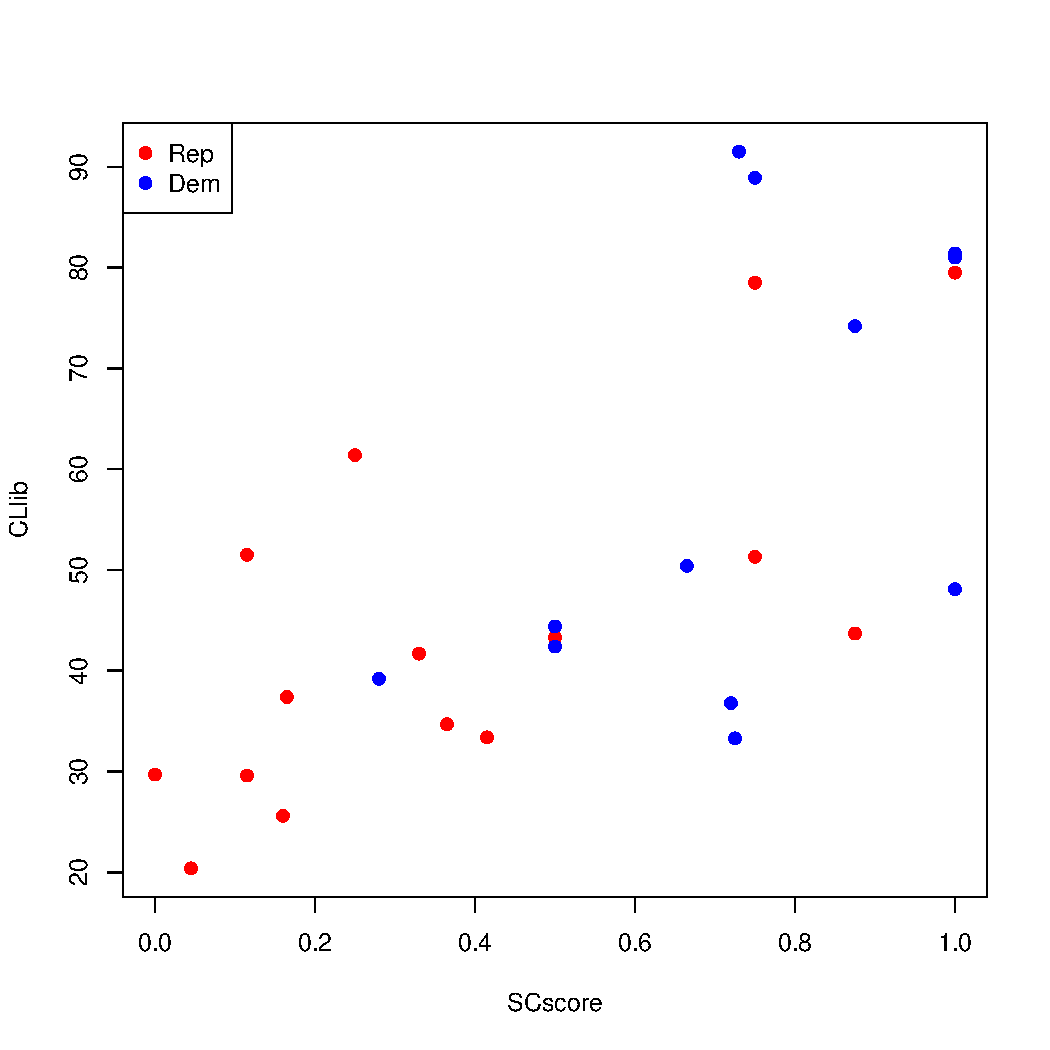
\includegraphics[width=3in]{psc.pdf}
%\end{figure}
%
%}
%
%\frame{
%\frametitle{One Binary and One Continuous Conditioning Variable}
%
%\begin{figure}[ht] \centering
%        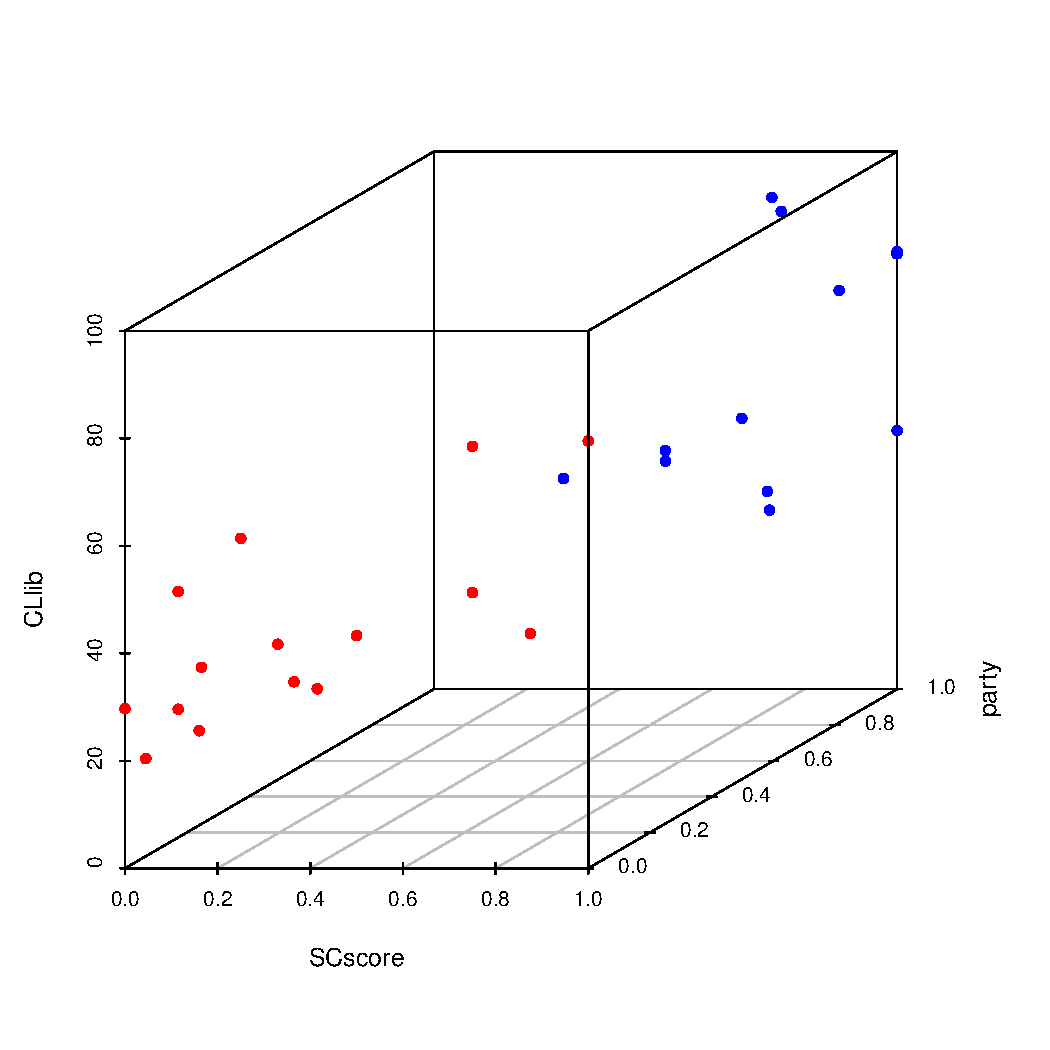
\includegraphics[width=3in]{em3D1.pdf}
%\end{figure}
%}
%
%\frame{
%\frametitle{One Binary and One Continuous Conditioning Variable}
%
%\begin{figure}[ht] \centering
%        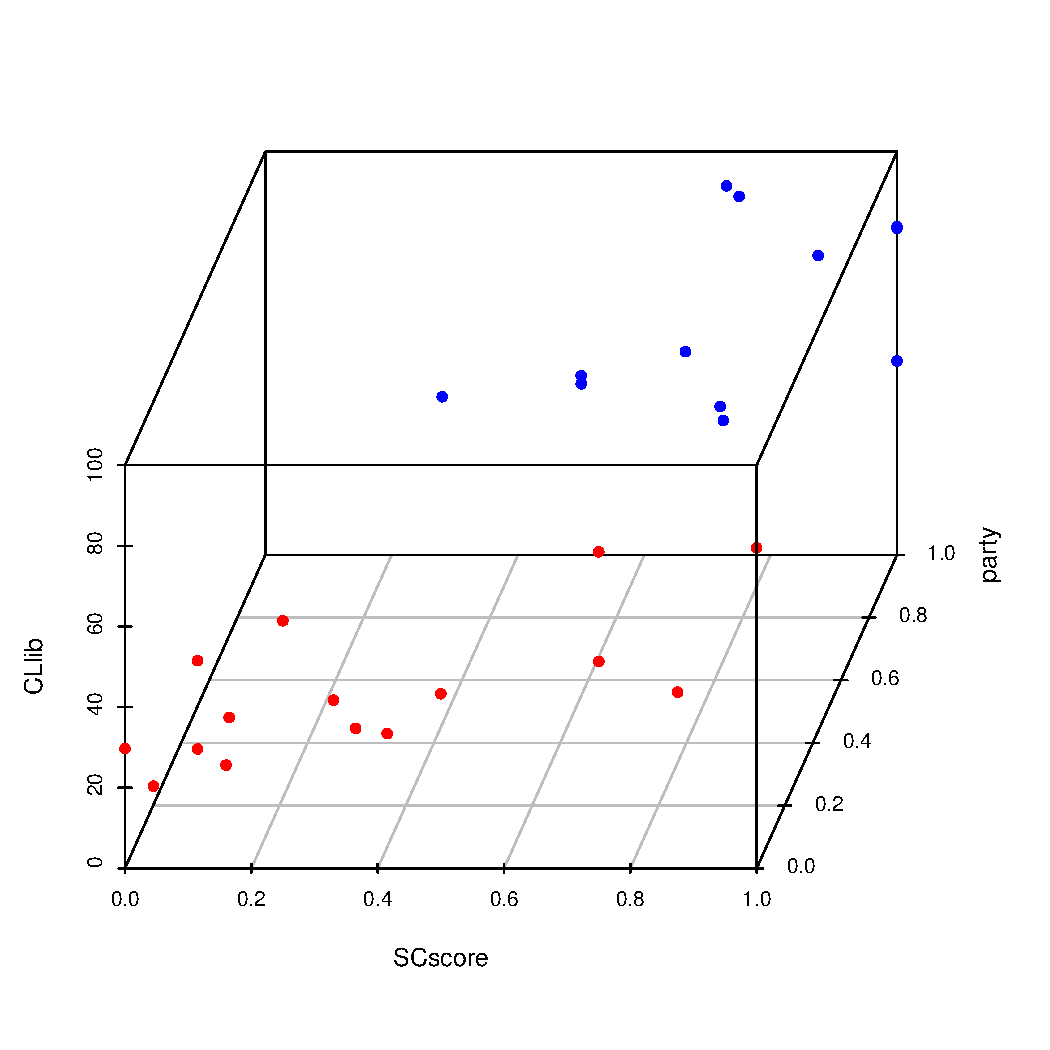
\includegraphics[width=3in]{em3D2.pdf}
%\end{figure}
%}
%
%\frame{
%\frametitle{Regression Plane}
%\begin{figure}[ht] \centering
%        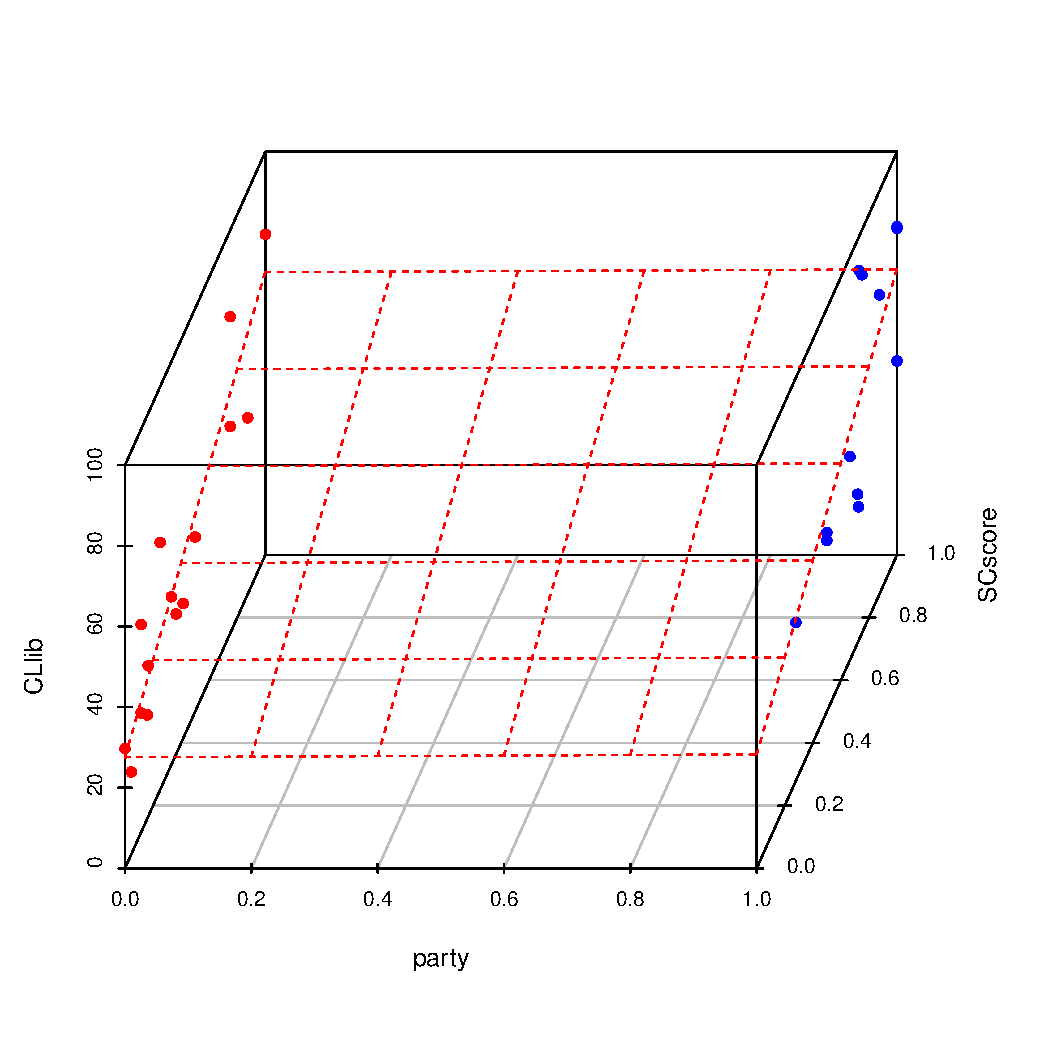
\includegraphics[width=3in]{em3D3.pdf}
%\end{figure}
%}
%
%\frame{
%\frametitle{Multiple Regression Activity}
%Draw the two regression lines (i.e., edges of the regression plane) implied by 
%$$
%\hat{y} = B_0 + B_1 x + B_2 z
%$$
%\begin{figure}[ht] \centering
%        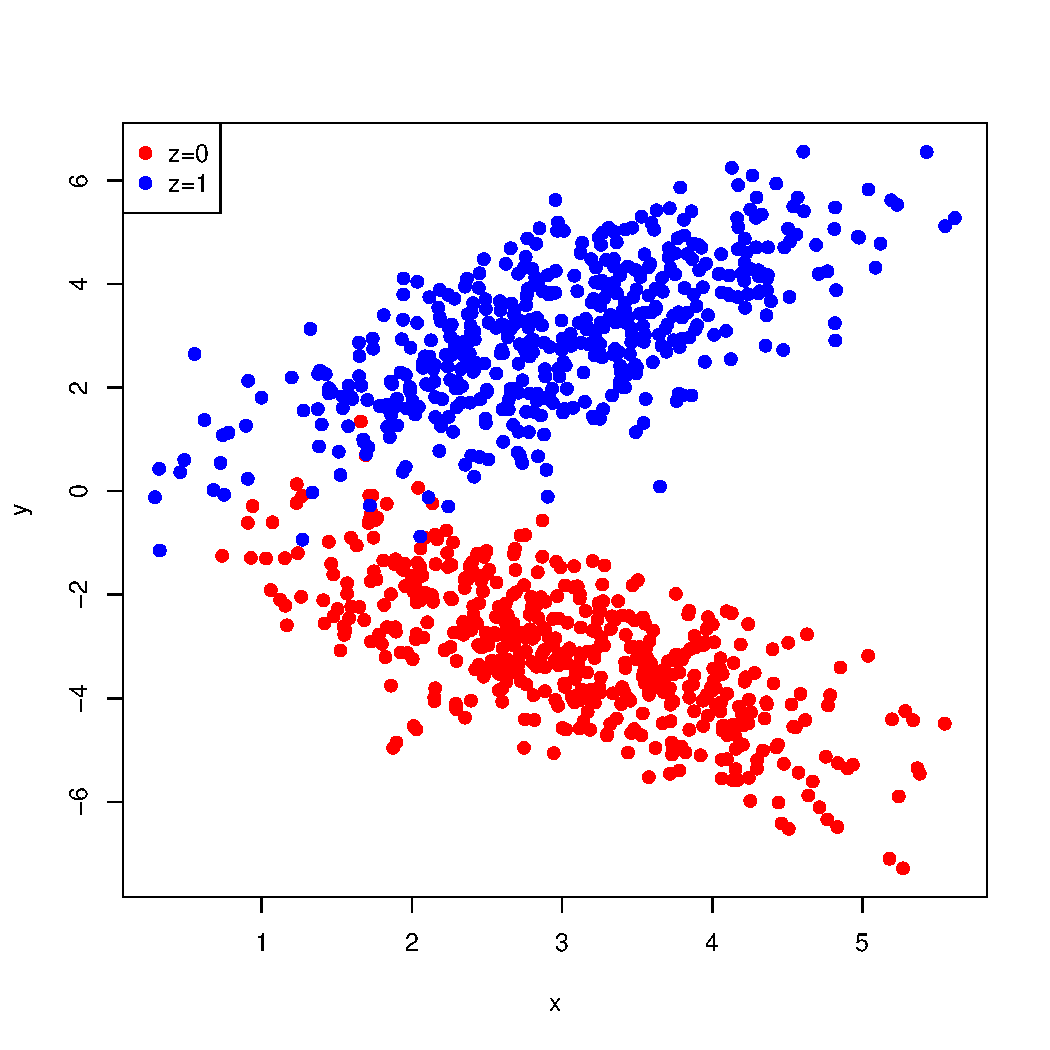
\includegraphics[width=2.5in]{multAct.pdf}
%\end{figure}
%
%}
%
%\frame{
%\frametitle{Multiple Regression Activity}
%Draw the two regression lines (i.e., edges of the regression plane) implied by 
%$$
%\hat{y} = B_0 + B_1 x + B_2 z
%$$
%\begin{figure}[ht] \centering
%        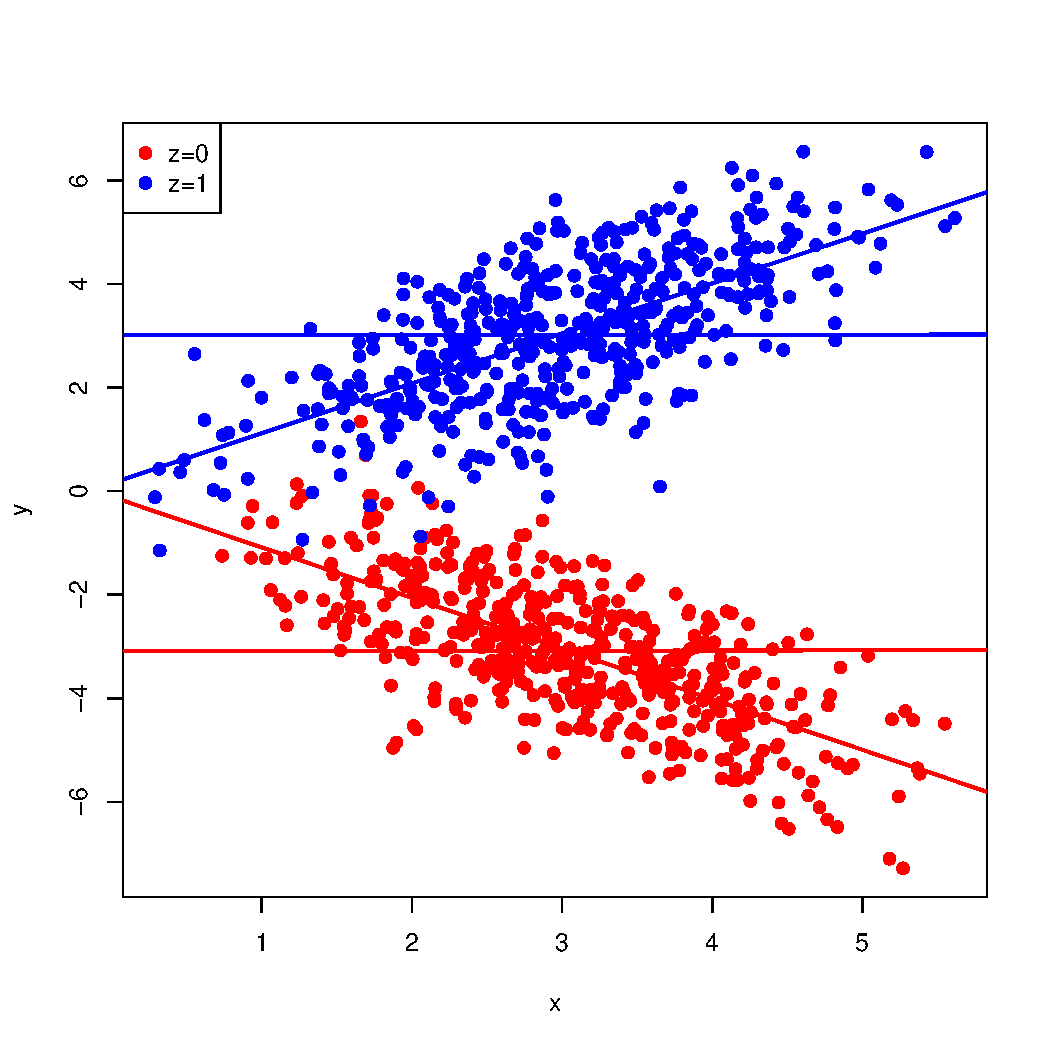
\includegraphics[width=2.5in]{multActSol.pdf}
%\end{figure}
%
%}
%
%
%\frame{
%\frametitle{Regression Plane for Two Continuous Conditioning Variables}
%
%\begin{figure}[ht] \centering
%        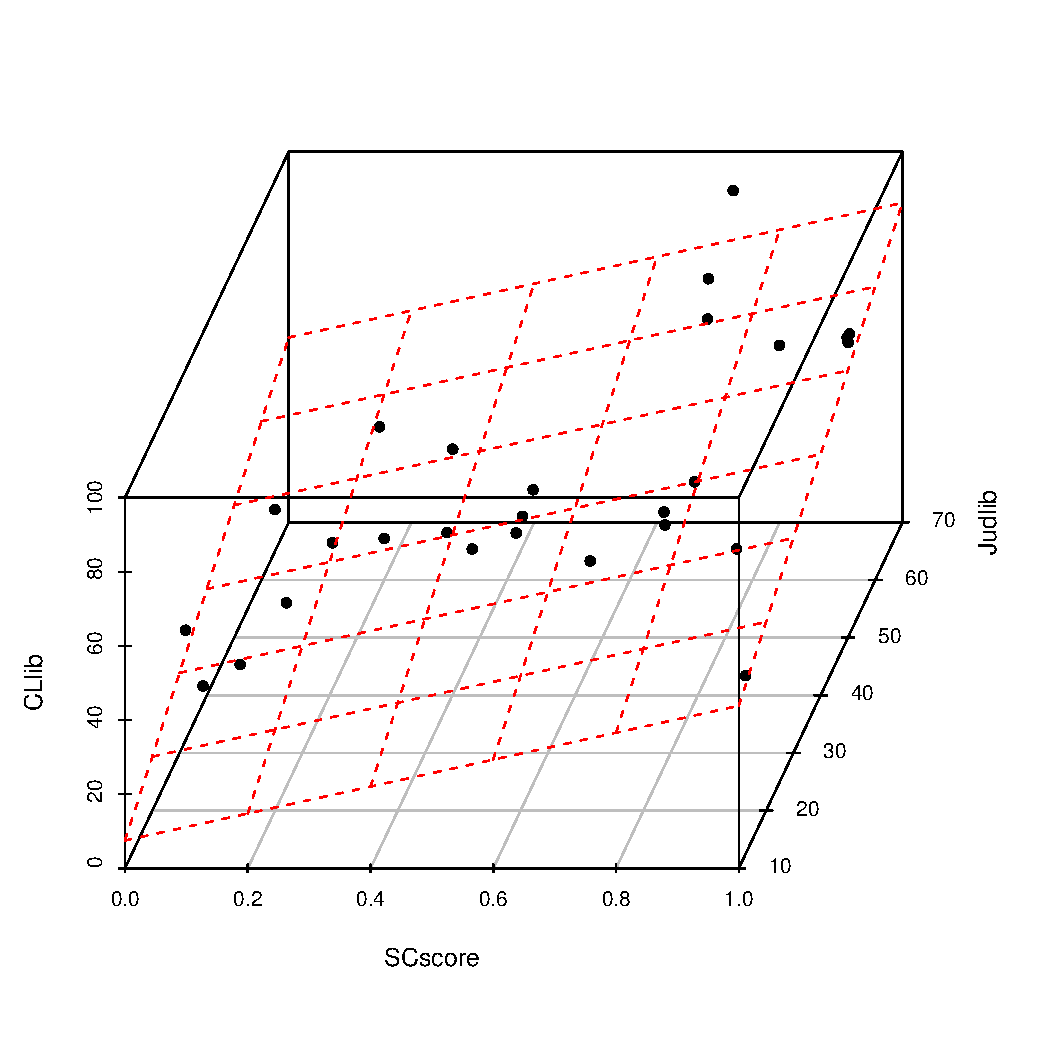
\includegraphics[width=3in]{em3D4.pdf}
%\end{figure}
%}
%
%
%\frame{
%\frametitle{Descriptive Interpretation of Additive Regression}
%
%$$\widehat{CLlib}_i = B_0 + B_1 \cdot SCscore_i + B_2 \cdot Dem_i$$
%
%\begin{figure}[ht] \centering
%        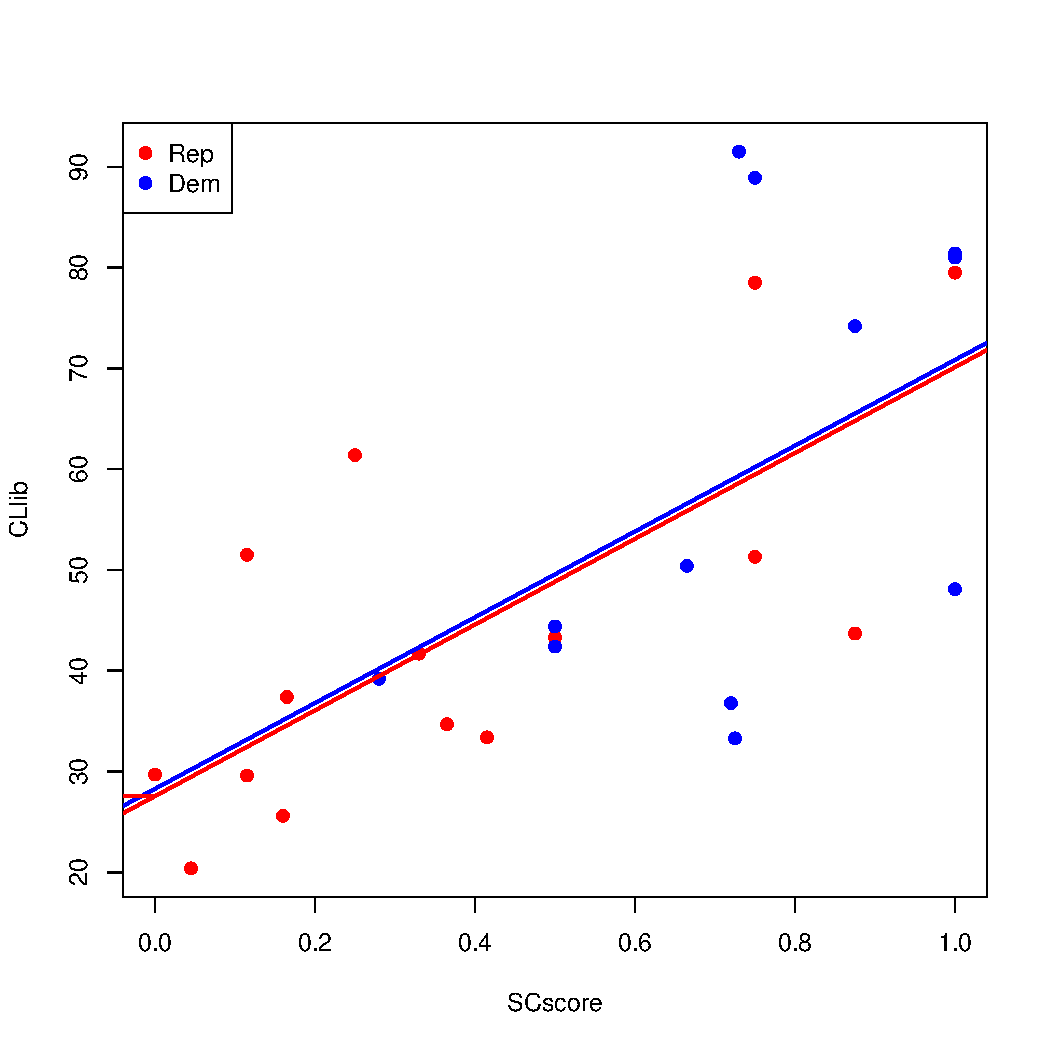
\includegraphics[width=2.7in]{pscMarg.pdf}
%\end{figure}
%
%}
%
%\frame{
%\frametitle{Recall: Simple Regression with SCscore}
%
%$$\widehat{CLlib}_i = B_0 + B_1 \cdot SCscore_i $$
%
%\begin{figure}[ht] \centering
%        \scalebox{.4}{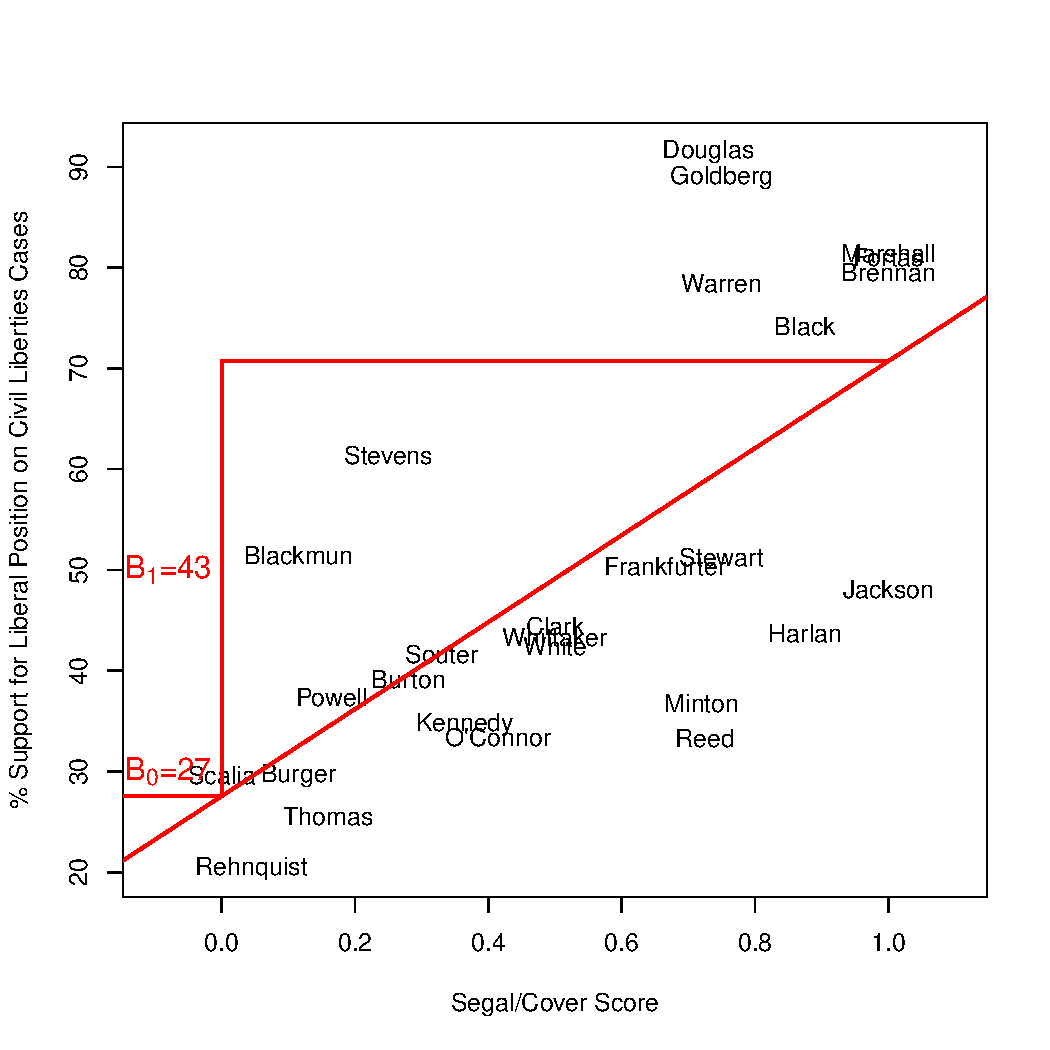
\includegraphics{lmPlot.pdf}}
%\end{figure}
%
%}
%
%\frame{
%\frametitle{Recall: Simple Regression with Party}
%
%$$\widehat{CLlib}_i = B_0 + B_1 \cdot Dem_i$$
%
%\begin{figure}[ht] \centering
%        \scalebox{.4}{
\includegraphics{lmBin.pdf}}
%\end{figure}
%
%
%}
%
%\frame{
%\frametitle{Descriptive Interpretation of Additive Regression}
%
%$$\widehat{CLlib}_i = B_0 + B_1 \cdot SCscore_i + B_2 \cdot Dem_i$$
%
%\begin{figure}[ht] \centering
%        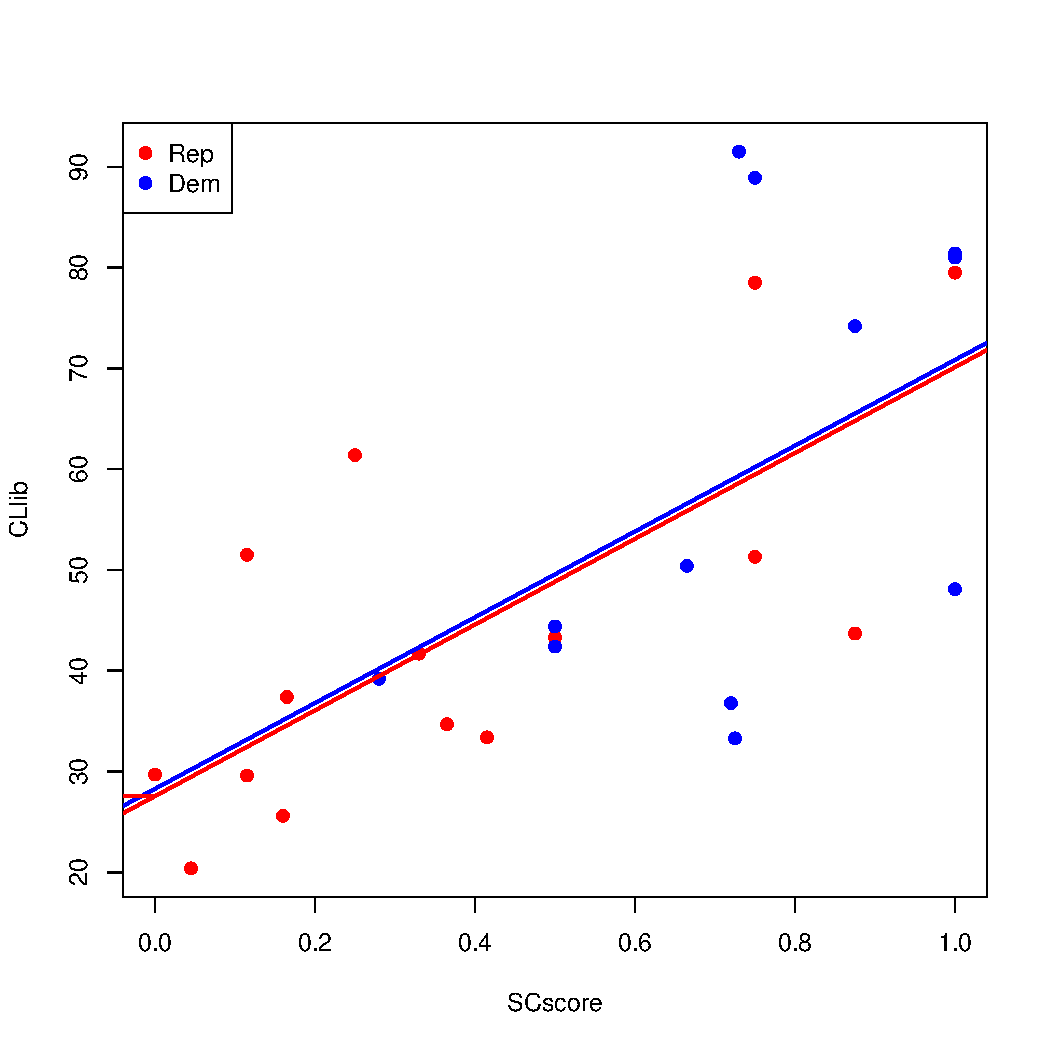
\includegraphics[width=2.7in]{pscMarg.pdf}
%\end{figure}
%
%}
%
%
%
%\frame{
%\frametitle{Descriptive Interpretation of Additive Regression}
%
%$$\widehat{Fedlib}_i = B_0 + B_1 \cdot SCscore_i + B_2 \cdot Dem_i$$
%
%\begin{figure}[ht] \centering
%      \includegraphics<1>[width=2.7in]{pscMarg2.pdf}
%	\includegraphics<2>[width=2.7in]{pscMarg20.pdf}
%	\includegraphics<3>[width=2.7in]{pscMarg21.pdf}
%	\includegraphics<4>[width=2.7in]{pscMarg22.pdf}
%	\end{figure}
%
%}
%
%\frame{
%\frametitle{Two reasons slope doesn't change}
%
%There are two reasons a slope doesn't change when including an additional variable in a regression
%
%\begin{itemize}
%\item if the original and additional control variables are uncorrelated
%\item if the slope for the additional variable in the multiple regression is zero
%\end{itemize}
%
%
%}
%
%
%\frame{
%\frametitle{Multiple Regression with an Interaction}
%
%\begin{itemize}
%\item Fitted Values: $\hat{y}_i = B_0 + B_1 x_i + B_2 z_i + B_3 x_i \cdot z_i$ \\
%for $i=1,...,N$ \pause
%\item Residuals:  $e_i = y_i - \hat{y}_i$ for $i=1,...,N$
%\end{itemize} \pause
%
%\vspace{.5cm}
%
%Again, we choose $B_0$, $B_1$, $B_2$, and $B_3$, to minimize the SSR, where
%\begin{align*}
%SSR &= \sum_{i=1}^N e_i^2
%\end{align*}
%but the definition of $e_i$ has again changed. 
%}
%
%
%
%
%\frame{
%\frametitle{Descriptive Interpretation of Interaction Model}
%
%$$\widehat{Fedlib}_i = B_0 + B_1 \cdot SCscore_i + B_2 \cdot Dem_i + B_3 \cdot SCscore_i \cdot Dem_i$$
%
%\begin{figure}[ht] \centering
%      \includegraphics<1>[width=2.7in]{pscInt.pdf}
%	\includegraphics<2>[width=2.7in]{pscInt0.pdf}
%	\includegraphics<3>[width=2.7in]{pscInt1.pdf}
%	\includegraphics<4>[width=2.7in]{pscInt2.pdf}
%	\includegraphics<5>[width=2.7in]{pscInt3.pdf}
%
%\end{figure}
%%
%}
%
%\frame{
%\frametitle{Variance and Multiple Regression}
%
%\begin{itemize}
%\item As before, we want to assess the ``leastness'' of  least squares (i.e., the spread of the data around the plane or twisted plane).
%\item The standard error of the regression, $\sqrt{\frac{\sum_{i=1}^N e_i^2}{N-k}}$, now accounts for the number of $B$'s in the model (where $k$ is the number of $B$'s).
%\item $R^2$ uses the same formula $1-\frac{SSR}{TSS}$, however the inclusion of additional variables will automatically reduce the SSR. 
%\end{itemize}
%
%}
%
%
%
%\frame{
%\frametitle{Summary Activity}
%
%\begin{figure}[ht] \centering
%      \includegraphics<1>[width=2.7in]{finalAct.pdf}
%	\includegraphics<2>[width=2.7in]{finalAct1.pdf}
%	\includegraphics<3>[width=2.7in]{finalAct2.pdf}
%	\includegraphics<4>[width=2.7in]{finalAct3.pdf}
%	\includegraphics<5>[width=2.7in]{finalAct4.pdf}
%\end{figure}
%
%}
%
%\frame{
%\frametitle{R Activity: Atlanta Science Festival Data}
%
%To Do:
%\begin{enumerate}
%\item Run regression of attendance on whether not free
%\item Run multiple regression of attendance on whether not free and estimated attendance
%\item Run multiple regression of attendance on interacted model
%\item Show the effect of shifting estimated attendance (e.g., subtracting off mean)
%\end{enumerate}
%
%
%
%}
%
%
%\frame{
%
%The FWL theorem and the meaning of "controlling" for an additional variable.
%
%}
%
%
%\frame{
%\frametitle{The Social Pressure Experiment}
%
%\begin{center}
%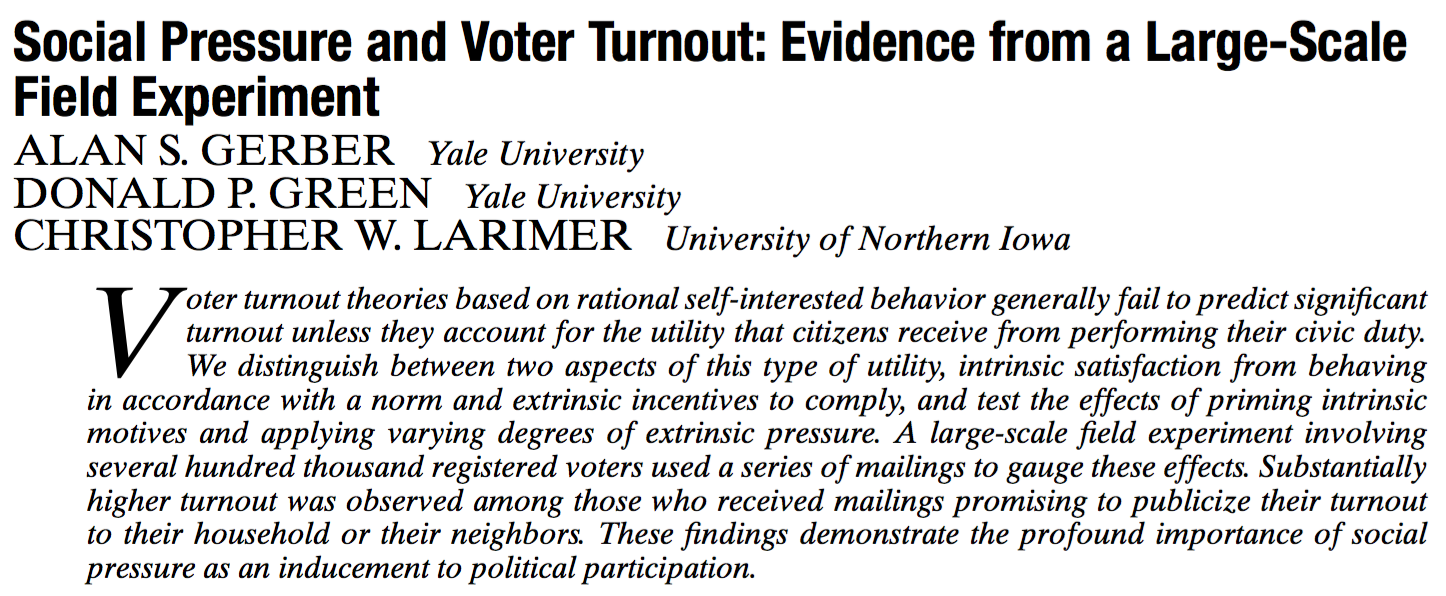
\includegraphics[width=4in]{abstractGGL}
%\end{center}
%
%}
%
%\frame{
%\frametitle{The Civic Duty Treatment}
%
%\begin{center}
%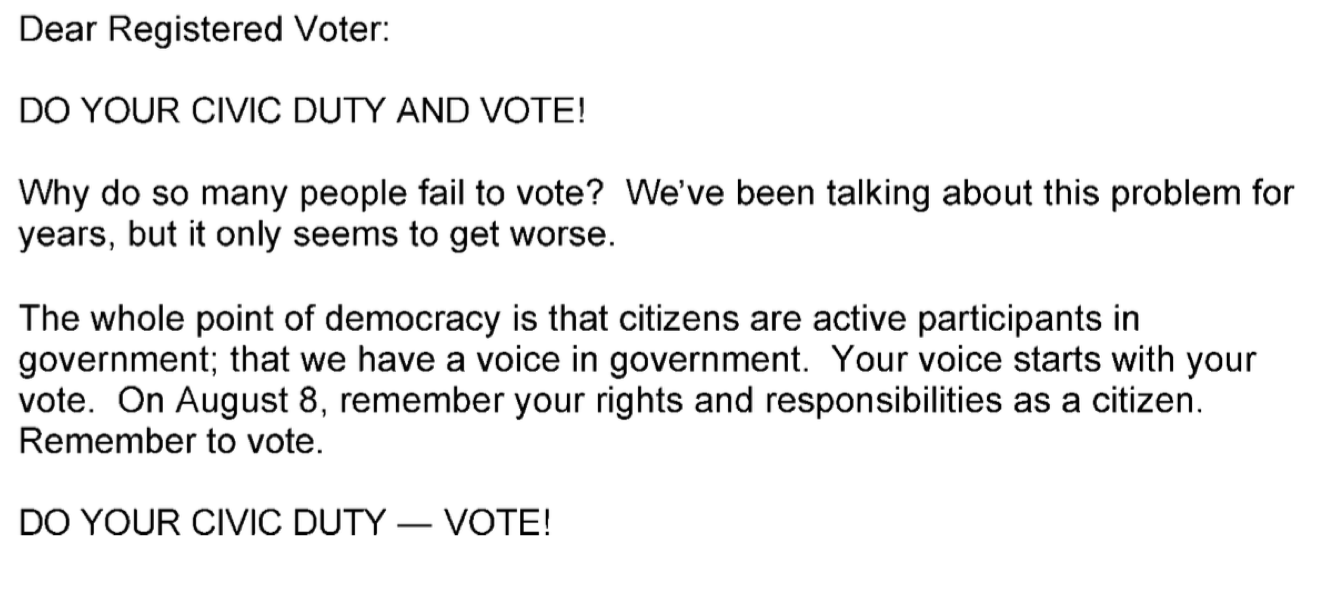
\includegraphics[width=4in]{CivicDutyGGL}
%\end{center}
%
%}
%
%\frame{
%\frametitle{The Hawthorne Treatment}
%
%\begin{center}
%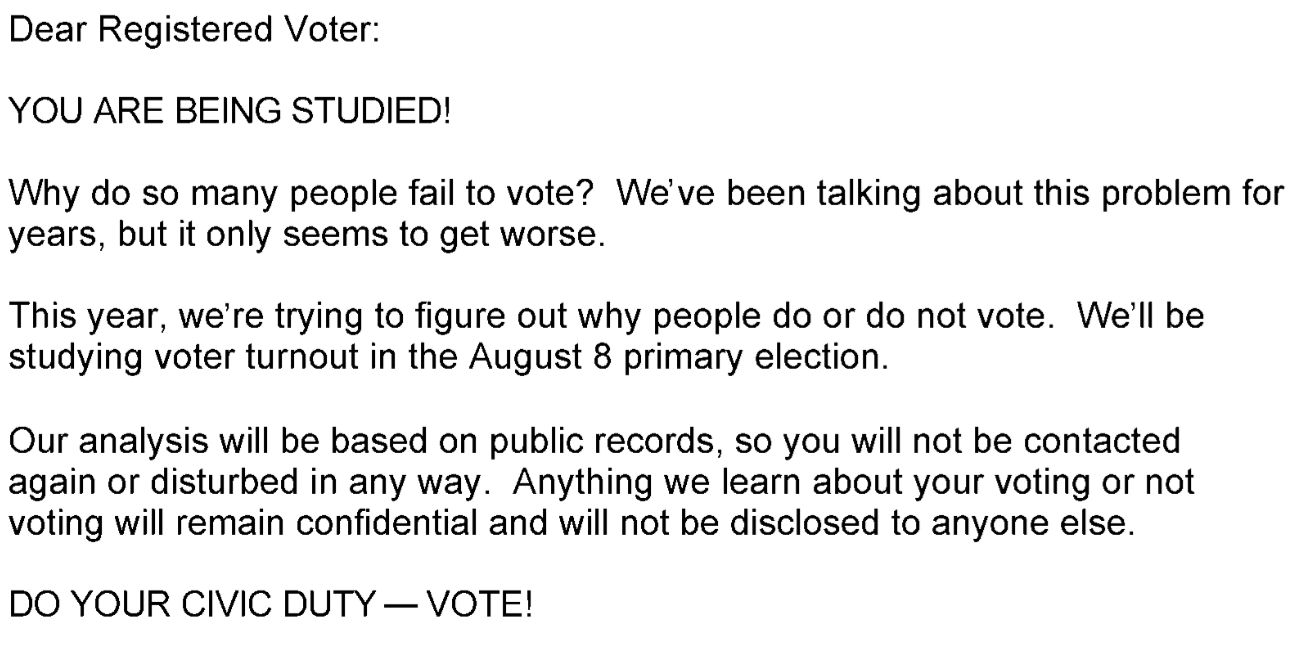
\includegraphics[width=4in]{HawthorneGGL}
%\end{center}
%
%}
%
%\frame{
%\frametitle{The Self Treatment}
%
%\begin{center}
%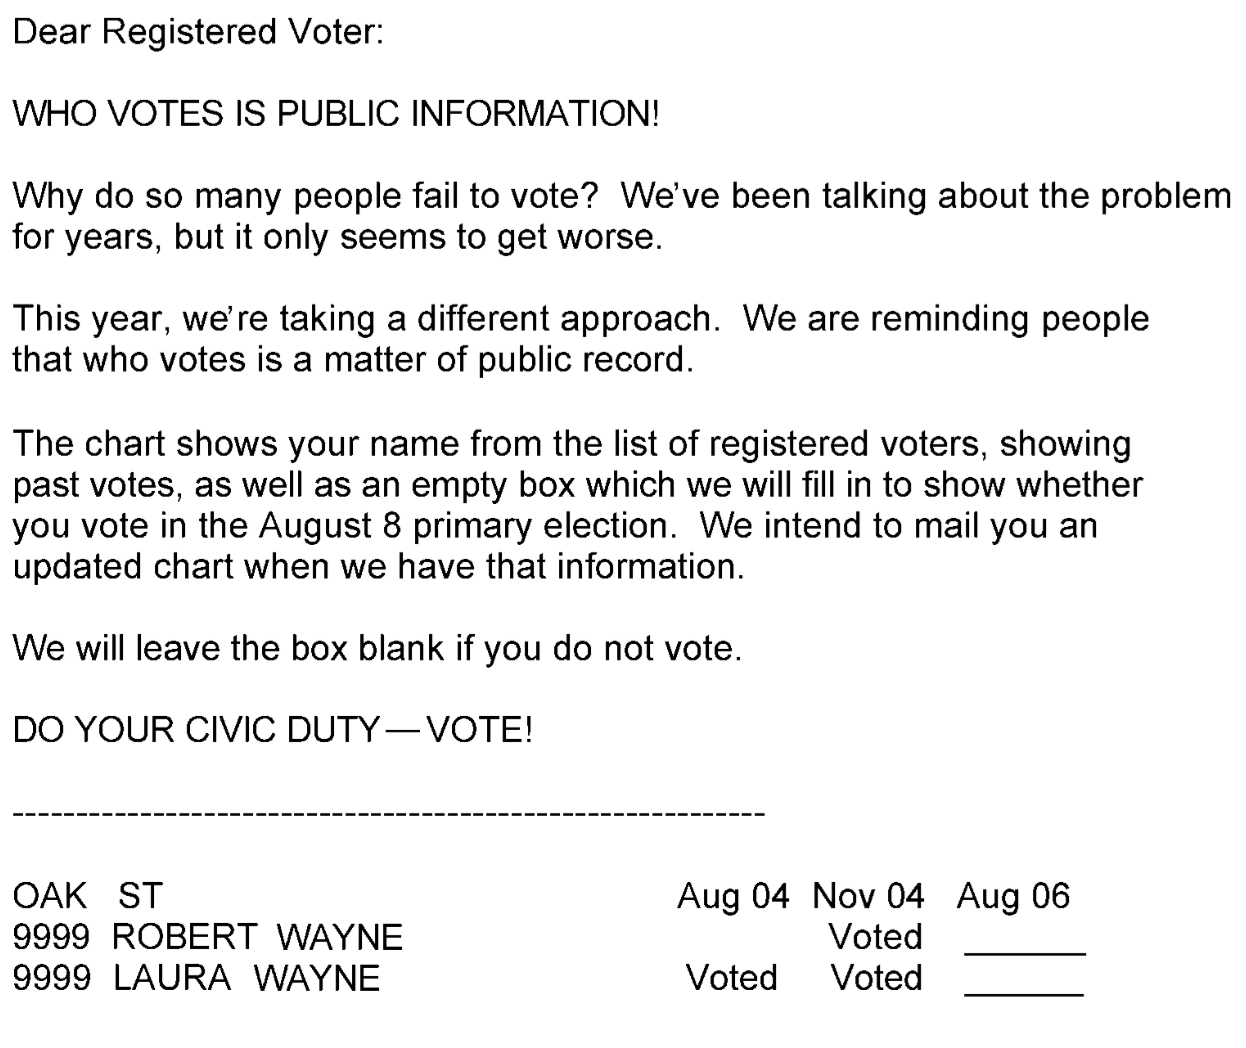
\includegraphics[width=3.5in]{SelfGGL}
%\end{center}
%
%}
%
%\frame{
%\frametitle{The Neighbors Treatment}
%
%\begin{center}
%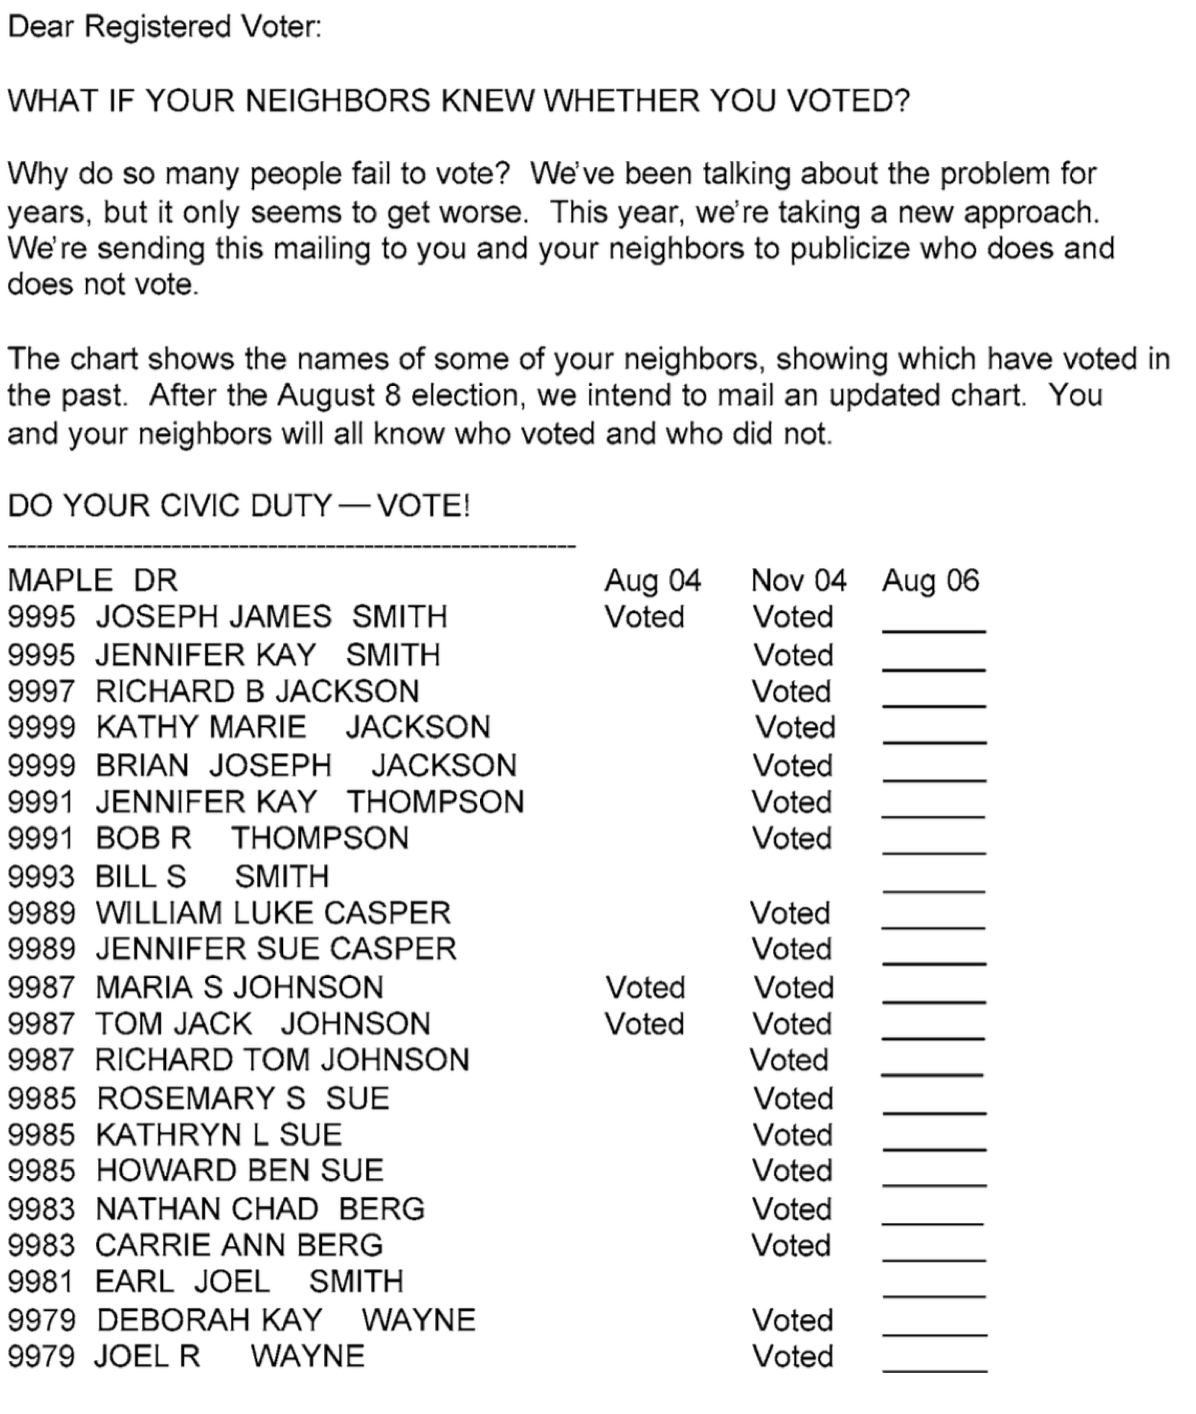
\includegraphics[width=3.5in]{NeighborsGGL}
%\end{center}
%
%}
%
%
%
%\frame{
%\frametitle{Balance on Pre-treatment Variables in the Gerber, Green, and Larimer Experiment}
%
%\begin{center}
%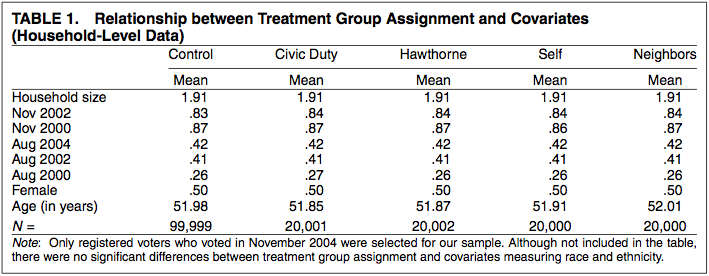
\includegraphics[width=4in]{GGL}
%\end{center}
%
%}
%
%
%\frame{
%\frametitle{Including Covariates in the Gerber, Green, and Larimer Experiment}
%
%\begin{center}
%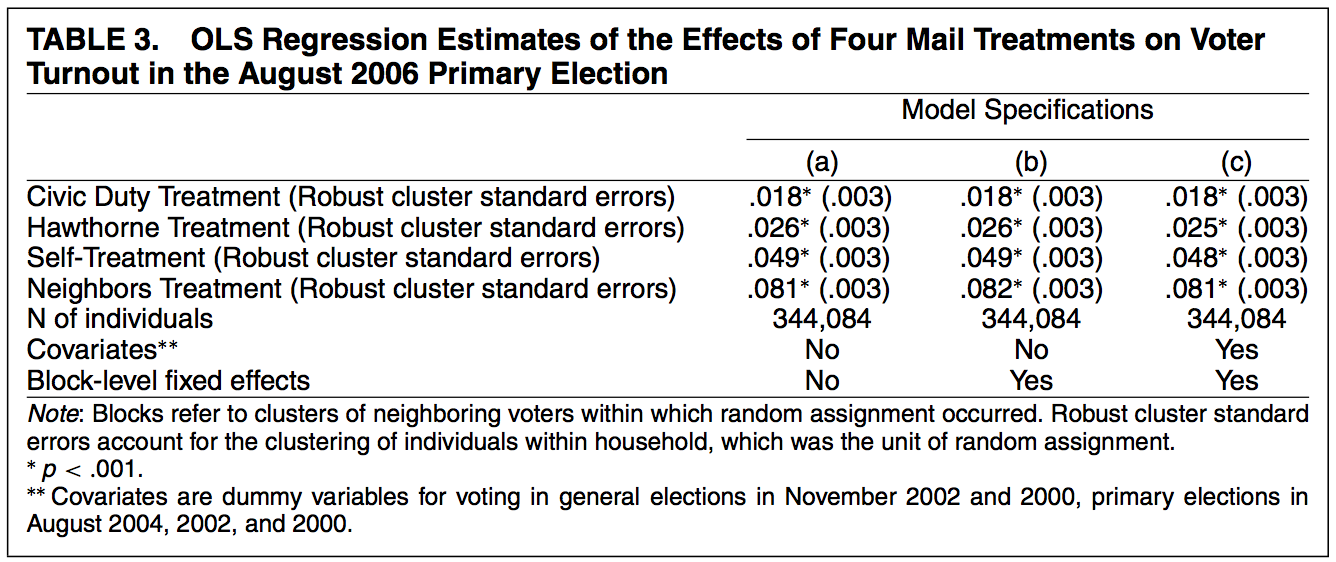
\includegraphics[width=4in]{GGL2}
%\end{center}
%
%}
%
%
%
%\begin{frame}
%\frametitle{FWL Theorem in Pictures}
%
%Results: $$\hat{\beta}_{X}^{Y \sim X+Z} = \hat{\beta}_{r_{X \sim Z}}^{r_{Y\sim Z} \sim r_{X\sim Z}}$$
%
%$$\hat{\beta}_{X}^{Y \sim X+Z} = \hat{\beta}_{r_{X\sim Z}}^{Y \sim r_{X\sim Z}}$$
%
%
%
%\end{frame}
%
%
%\begin{frame}[fragile]
%\frametitle{Simulating Linear Model Data}
%
%\begin{verbatim}
%> n <- 10000
%> set.seed(1234)
%> z <- rnorm(n)
%> x <- z + rnorm(n)
%> y <- x + z + rnorm(n)
%> cor(x,z)
%[1] 0.7044271
%\end{verbatim}
%
%\end{frame}
%
%\begin{frame}[fragile]
%\frametitle{Linear Regression Output}
%
%\begin{verbatim}
%> lm(y ~ x)
%
%Coefficients:
%(Intercept)            x  
%    0.01099      1.48301  
%
%> lm(y ~ x + z)
%
%Coefficients:
%(Intercept)            x            z  
%    0.00417      0.99901      0.98608 
%\end{verbatim}
%
%\end{frame}
%
%\begin{frame}[fragile]
%\frametitle{Added Variable ``Plot'' (Partial Regression ``Plot'')}
%
%\begin{verbatim}
%> r_yz <- residuals(lm(y ~ z))
%> r_xz <- residuals(lm(x ~ z))
%> r_yxz <- residuals(lm(y ~ x+z))
%> lm(r_yz ~ r_xz)
%
%Coefficients:
%(Intercept)         r_xz  
% -3.619e-16    9.990e-01  
%
%> range(r_yxz - residuals(lm(r_yz ~ r_xz)))
%[1] -2.211564e-13  4.019007e-14
%\end{verbatim}
%
%\end{frame}
%
%
%\begin{frame}[fragile]
%\frametitle{Only $x$ residualized}
%
%\begin{verbatim}
%> lm(y ~ r_xz)
%
%Coefficients:
%(Intercept)         r_xz  
%   0.008571     0.999006  
%
%> range(r_yxz - residuals(lm(y ~ r_xz)))
%[1] -7.209635  6.790846
%\end{verbatim}
%
%\end{frame}
%
%\frame{
%What if $x$ and $z$ are uncorrelated?
%
%\bigskip
%
%What if $x$ and $z$ perfectly correlated?
%
%}
%
%\frame{
%What if $x$ and $z$ are uncorrelated?
%
%\bigskip
%
%$$\hat{\beta}_{X}^{Y \sim X} = \hat{\beta}_{X}^{Y \sim X + Z}$$
%
%\ \ \ \ \ \ \ \ \ \ \ \ \ \ \ \ \ \ \ \ \ \ \ \ \ \ \ \ \ \ \ \ \ \ \ \ \ \ \ \ Why? (see whiteboard) 
%
%\bigskip
%
%What if $x$ and $z$ perfectly correlated?
%
%}
%
%\frame{
%What if $x$ and $z$ are uncorrelated?
%
%\bigskip
%
%$$\hat{\beta}_{X}^{Y \sim X} = \hat{\beta}_{X}^{Y \sim X + Z}$$
%
%\ \ \ \ \ \ \ \ \ \ \ \ \ \ \ \ \ \ \ \ \ \ \ \ \ \ \ \ \ \ \ \ \ \ \ \ \ \ \ \ Why? (see whiteboard) 
%
%\bigskip
%
%What if $x$ and $z$ perfectly correlated?
%
%\ \ \ \ \ \ \ \ \ \ \ \ \ \ \ \ \ \ \ \ \ \ \ \ \ \ \ \ \ \ \ \ \ \ \ \ \ \ \ \ We can't fit a regression! 
%
%}
%
%
%
%\begin{frame}[fragile]
%\frametitle{What if $x$ and $z$ are uncorrelated?}
%
%\begin{verbatim}
%> z <- rnorm(n)
%> x <- rnorm(n) # no z
%> cor(x,z)
%[1] 0.01075281
%> y <- x + z + rnorm(n)
%> lm(y ~ x)
%Coefficients:
%(Intercept)            x  
%    0.01027      1.00940  
%
%> lm(y ~ x + z)
%
%Coefficients:
%(Intercept)            x            z  
%    0.00417      0.99901      0.98509  
%    \end{verbatim}
%
%\end{frame}
%
%\frame{
%\frametitle{A simple proof of the $x$-only version}
%
%\begin{align*}
%y &= \beta_0 + \beta_1 x + \beta_2 z + \epsilon \\
%x &= \alpha_0 + \alpha_1 z + v
%\end{align*}
%
%
%
%\begin{align*}
% \frac{Cov(y,r_{x\sim z})}{V(r_{x\sim z})} &=\frac{Cov(\beta_0 + \beta_1 x + \beta_2 z + \epsilon,v)}{V(v)}\\
%&=\frac{Cov(\beta_0,v) + Cov(\beta_1 x,v) + Cov(\beta_2 z,v) + Cov(\epsilon,v)}{V(v)}
%\end{align*}
%
%}
%
%\frame{
%\frametitle{Simple proof continued}
%
%\begin{align*}
%\frac{Cov(\beta_1 x,v)}{V(v)} &=\frac{Cov(\beta_1(\alpha_0 + \alpha_1 z +v), v)}{V(v)}\\
%  &=\frac{Cov(\beta_1 \alpha_0,v) + Cov(\beta_1 \alpha_1 z,v) + Cov(\beta_1 v, v)}{V(v)}\\
%  &=\frac{0 + 0 + \beta_1 Var(v)}{Var(v)}\\
%  &=\beta_1
%\end{align*}
%
%}
%
%
%\frame{
%\frametitle{Next Week}
%
%What changes for nonlinear models (e.g., logistic regression)?
%
%}
%
%%\frame{
%%\frametitle{Summary}
%%
%%\begin{itemize}
%%\item There are many possible descriptive questions with many variables and variables that take many values. 
%%\item In this course we focus on means (possibly conditional), although variance and standard deviation are also concerns. 
%%\item Conditioning requires modeling choices. In this course we use linear models (with and without interactions). 
%%\end{itemize}
%%
%%}
%%
%%\frame{
%%\frametitle{Next Week}
%%
%%Randomly Sampled Observations and Basic Probability
%%
%%\begin{itemize}
%%\item Elementary Probability Theory
%%\item Random Variables and Functions of Random Variables (Expectation, Variance, ...)
%%\item Joint and Conditional Distributions
%%\end{itemize}
%%
%%\vspace{.5cm}
%%
%%Things to do:
%%\begin{itemize}
%%\item first problem set
%%\item the reading and the reading quiz
%%\item annotations (if you have a question or want to respond to a question)
%%\end{itemize}
%%
%%
%%
%%}



\end{document}












